\documentclass[10pt, conference]{IEEEtran}

\usepackage{amsmath,amssymb,amsfonts}
\usepackage{algorithmic}
\usepackage{graphicx}
\usepackage{textcomp}
\usepackage{xcolor}
\usepackage{hyperref}
\usepackage{listings}
\usepackage[backend=biber]{biblatex}
\addbibresource{mycite.bib}
\def\BibTeX{{\rm B\kern-.05em{\sc i\kern-.025em b}\kern-.08em
    T\kern-.1667em\lower.7ex\hbox{E}\kern-.125emX}}
\begin{document}

\title{Automatic Detection of Cryptographic API Misuses in Stack Overflow Java Code Snippets\\}

\author{\IEEEauthorblockN{Kristen Newbury}
\IEEEauthorblockA{University of Alberta \\
knewbury@ualberta.ca}
}

\lstset{ %
  backgroundcolor=\color{white},   % choose the background color
  basicstyle=\footnotesize,        % size of fonts used for the code
  breaklines=true,                 % automatic line breaking only at whitespace
  captionpos=b,                    % sets the caption-position to bottom
  commentstyle=\color{mygreen},    % comment style
  escapeinside={\%*}{*)},          % if you want to add LaTeX within your code
  keywordstyle=\color{blue},       % keyword style
  stringstyle=\color{mymauve},     % string literal style
}


\maketitle

\begin{abstract}
Stack Overflow (SO) is a valuable platform for information for application developers. For this reason it is impertinent that the software development community considers the utility of code snippets distributed on the platform with a variety of metrics of software quality in mind. One crucial, but easily overlooked, metric of software quality is security. 

Recent work has applied manual classification to determine the security status of SO snippets. Other  work has applied machine learning to determine the security of code snippets on SO. There has also been work using static analysis on Android applications on Google Play that are considered to contain SO code snippets. No previous work has applied static analysis to accomplish automatically detecting insecure versions of Stack Overflow (SO) code snippets with respect to Cryptographic API usage.

In this study we aim to assess the viability of automating assessment of security directly on code snippets using a static analysis tool, CogniCrypt. We have extracted a sample of Java code snippets that use the cryptographic API, JCA, from SO and evaluated this sample of snippets to determine if there are misuses of cryptographic APIs present. We have found that approximately 50\% of the code snippets we were successful applying a relevant analysis to contained insecure usage of cryptographic APIs. 
\end{abstract}

\section{Introduction}
SO code snippets can be categorized as secure or insecure based on the viability of the code as a solution to security related task. Insecurity in SO code snippets have a great implication. This is because it can be hard to concretely measure the cascading impact of an individual code snippet. 
Clearly posts with more views and answers that are accepted can be seen as sources of information with a higher likelihood of reaching many locations of use, but if  these end locations are proprietary, or if a snippet is pasted into code that is subsequently reused, it may be hard to trace eventually arising faults to the SO snippet.

Previous work \cite{Egele:2013:ESC:2508859.2516693} has looked at reasons that insecurity can arise in applications programming, specifically in terms of API usage. One insight of this study was that official API documentation can be lengthy and complex or non-present or insufficient as a resource for developers who are required to perform particular software development tasks. Another insight from this study is that misuse was prevalent in high percentage (88\%) of the Android applications that the study analyzed. 

Another previous study \cite{7546508} has found that SO has potential to be a valuable alternative source of information for developers. In a software development world where deadlines are real and efficiency of development processes are championed, SO is an attractive software development resource as it can enable developers to perform tasks quickly and efficiently. However, the same study also has found that it may not be the best source of information when it comes to performing security related application tasks.


A discussion of an ideal solution to assessing SO code snippet security is presented by in this work \cite{DBLP:journals/corr/abs-1901-01327}. In this work it is concluded that an ideal solution would be to have a full automation of secureness classification. This ideal solution could be applied in two potential ways: as a check on the existing corpus of SO code snippets, with the possible goal of one of the following: alerting the author of the post to their presence, automatically tagging the post with a warning, or suggesting a fix. Another suggested outcome of such a work would be to integrated such a tool into the workflow of submission of posts to SO. The idea here is that the user submits a post, and in almost instant time the post is assessed for secureness and feedback is delivered if the post is insecure. Perhaps the submission is even rejected. In particular this second usage of such a pipeline tool could foster an awareness for good security practices in the software development community. While this work has not addressed either of these two goals directly, we believe that it would be viable to apply the work done here in either of these settings.

Additionally a few recent works have focused on the nature of code snippets on SO. \cite{7958574} has used machine learning (ML) to classify security of code snippets. In order to train their ML model they manually label 1,360 snippets as secure or insecure. They also perform a static analysis on Android applications on Google Play, and make an argument about the strength of connection between these snippets and the analyzed applications based on a graph similarity comparison over Program Dependency Graphs constructed from the snippets. Other work has been done on the security of code snippets on SO \cite{DBLP:journals/corr/abs-1901-01327}. This work seems to be over the largest data sample to date and has performed a manual analysis of the security of 8,690 snippets. However unlike our own work the previous two have a significant amount of manual effort involved. While both studies mention using multiple authors and open discussions to determine the labelling of snippets, they do not present an inter-rater reliability metric, and despite this, in order to replicate their exact results a great amount of manual effort would again be required. In this study we aim to pipeline the process, such that anyone with access to the data would at least be able to obtain our results easily.

One other study, \cite{Zhang:2018:CEO:3180155.3180260} looks at the reliability of code examples on SO in terms of API usage in general. The tool used in this study, ExampleCheck operates on a control flow graph (CFG) therefore bypassing the need and complexity for partial program compilation.
 
 
Lastly we must acknowledge the inherently multifaceted nature of the notion of security. Security is complex, in that every layer of a system is affected by it, and even within layers there are multiple dimensions to the notion of security. One previous work \cite{Yang2016} has observed that there are five main topics relating to security discussions in SO, some of these topics include web security, system security and cryptography. In this study we restrict our focus to application security, and specifically cryptographic security, via an evaluation of cryptographic API usage.

We classified security of code snippets concretely as either the presence or lack thereof cryptographic API misuses. We used the static analysis tool CogniCrypt \cite{krger_et_al:LIPIcs:2018:9215} to detect misuses. CogniCrypt is a static analysis tool that performs upon compiled Java bytecode that use cryptographic APIs and assess whether there exists some misuses of the API. Misuse is defined in a Domain Specific Language as a set of specifications over the entities that are relevant to that API. CogniCrypt is distributed with a ruleset for the Java Cryptography Architecture (JCA). The JCA is an architecture facilitating a standardized distribution of cryptographic task implementations.

In this work we aim to automate the analysis steps of collecting, filtering, preprocessing, compiling and analyzing Java code snippets utilizing a cryptographic API. We use a series of textual search and preprocessing techniques, followed by compilation using Soot PPA, and lastly analysis performed by the static analysis tool, CogniCrypt.


In order to complete this goal we have formulated the following research questions.
\begin{itemize}
 \item  RQ1: Do cryptographic API misuses exist in code snippets from Stack Overflow?

\item  RQ2: What is the most common error detected in code snippets?

\item  RQ3: Can we estimate the impact of insecurity of code snippets?

\end{itemize}

We make our work publicly accessible in the following Github repository:
\url{https://github.com/knewbury01/SnipPipeServe}


\section{Methodology Overview}

\begin{figure}[h]
\begin{center}
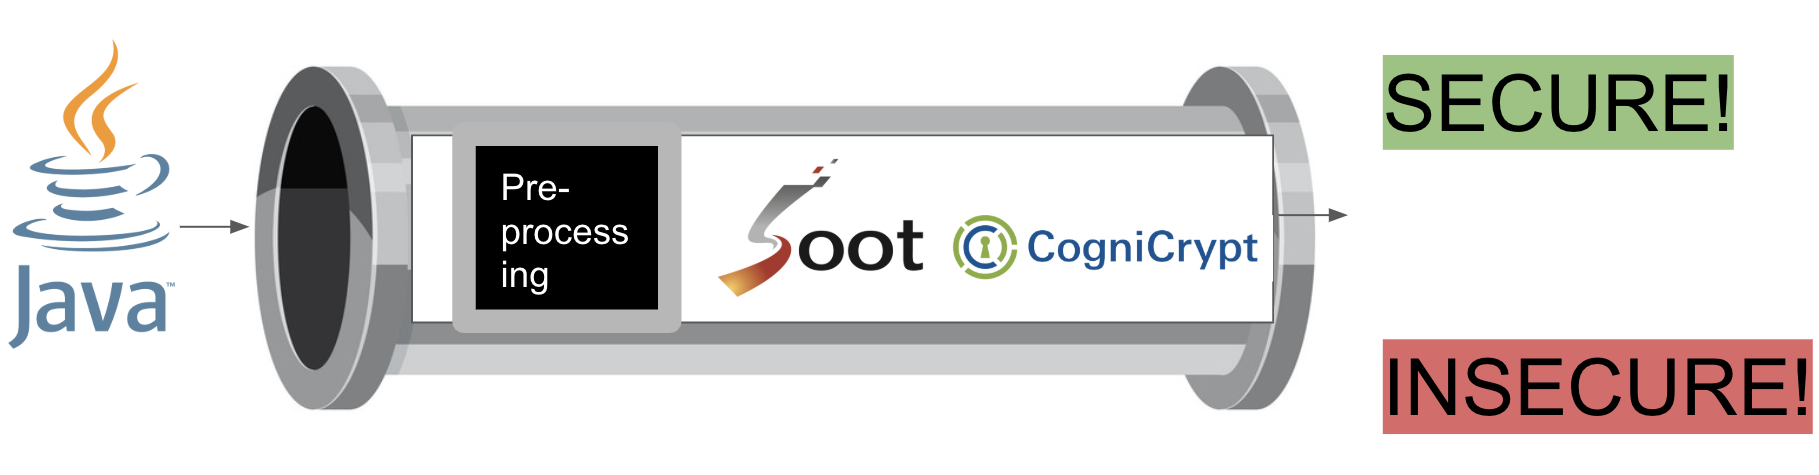
\includegraphics[width=1.0\linewidth]{pipeline.png}
\caption{Highlevel overview of process to assess snippets}
\end{center}
\end{figure}

In order to produce an labelling of secureness of code snippets, we first identify a relevant sample of SO code snippets to assess. Relevant is defined in terms of the tools used in this study. We are constrained to Java code snippets performing tasks that utilize cryptographic APIs, that additionally compile. First we extract relevant snippets, which are fed into a pipeline, with three main stages: preprocessing, compilation and analysis. Based on the output of the analysis we assess a snippet as insecure or secure based on the presence or lack thereof, respectively, of an error as reported by CogniCrypt.

\section{Tool Versions}

We strongly believe in the replicability of studies, as such we detail here the versions of tools used in our process such that any interested reader should be able to replicate as much of the setup of the study as possible.

The build of CogniCrypt that was used in this study roughly corresponds to release 2.0.0, but specifically was obtained from commit sha: 5f531d1d4377aefd35cec6658ae95308c6594244. The JCA ruleset was obtained as the zip download from release 2.0.0. 

Soot' partial program analysis (PPA) tool v0.1 \cite{SootPPA} was used to perform compilation. One caveat of using this tool is that it is no longer maintained, and as such only provides full support of Java features for up to Java 1.4. We were required to make some source code changes to snippets to deal with such, as discussed below. These changes would not affect the semantics of the analysis that CogniCrypt performs.

The rt.jar file that we supplied to Soot PPA (since it assumes a Java 1.4 environment) was from this exact Java SE Development Kit, j2sdk14202solarisi586, 
obtained here 
\url{https://www.oracle.com/technetwork/java/javasebusiness/downloads/java-archive-downloads-javase14-419411.html} .

\section{Dataset and Snippet Sample Collection}


From this point we must define relevant code snippets for this study as code snippets containing Java code only, since CogniCrypt performs analysis upon Java bytecode. There is also the resulting requirement that the code snippets must be compilable. The previous studies that we have mentioned earlier that handle code snippet analysis of any sort have relied upon either AST or IR representation of the snippets, as the lowest level representation handled. They did not require the snippets to be compiled. This presents an additional complexity to our study. Code snippets, by definition, are partial programs. They often do not contain sufficient context to compile. Below we discuss in further detail the efforts necessary to deal with this, however these insights guide the rest of the data processing steps.

The dataset used for SO snippet collection this study was an sqlite import \cite{wong_2019} of the SOTorrent dataset released previously in an MSR submission \cite{DBLP:conf/msr/BaltesDT008}. In order to evaluate security of code snippets with CogniCrypt we collected snippets related to both security and java. 

In gathering data we performed the following steps in order to gather a relevant and reasonable set of code snippets to evaluate.

\subsection{Identifying Answer Posts Containing Java Security Snippets}
In the process of identifying java code snippets, only snippets from answer posts were considered. This was because of the intuition that answer posts are more likely to be a source for code that will be copied into a project, as noted in previous work \cite{7958574}. Code snippets were identified as Java Security related if they originated from answers to posts that were labelled with the both the “java” and "security" tag on Stack Overflow. Posts annotated with java-ee and java-se were not explicitly sought out, from the intuition that posts with these tags mostly also had the java tag as well. As well, only accepted answers posts were considered, as it can be argued that the answer that will be utilized the most will be the accepted answer, and that often the rest of the answers are less utilized. Only the latest version of a post was examined, as this is assumed to fairly represent what an author intended to share at that time. Analysing previous versions of a post would not be fair because bug fix edits may have been made to a post at some point in time, and separately modelling all versions of posts would not realistically give us an indication of overall security at one point in time. Finally, each code block of a post is treated as a separate snippet.  


\subsection{Identifying Crypto Security Related Posts}
In order to collect usages of crypto APIs specifically, considering that CogniCrypt uses a ruleset tailored to the JCA, we also filtered our dataset for snippets using a particular set of keywords. 
Normally a reasonable process to identify API usage of a piece of java software would be to look at the import statements listed in the project, however because of the partial nature of code snippets this technique would not work. We found that only approximately 6\% of the code snippets of our sample contained at least one import. It is likely that SO authors assume that the user of the code snippet can obtain the resolution of Objects themselves, and that they will supply the missing import statement.
In order to then identify usages of cryptographic libraries we only retained code snippets that contained at least one of the following keywords.

\begin{table}[h]
\begin{center}
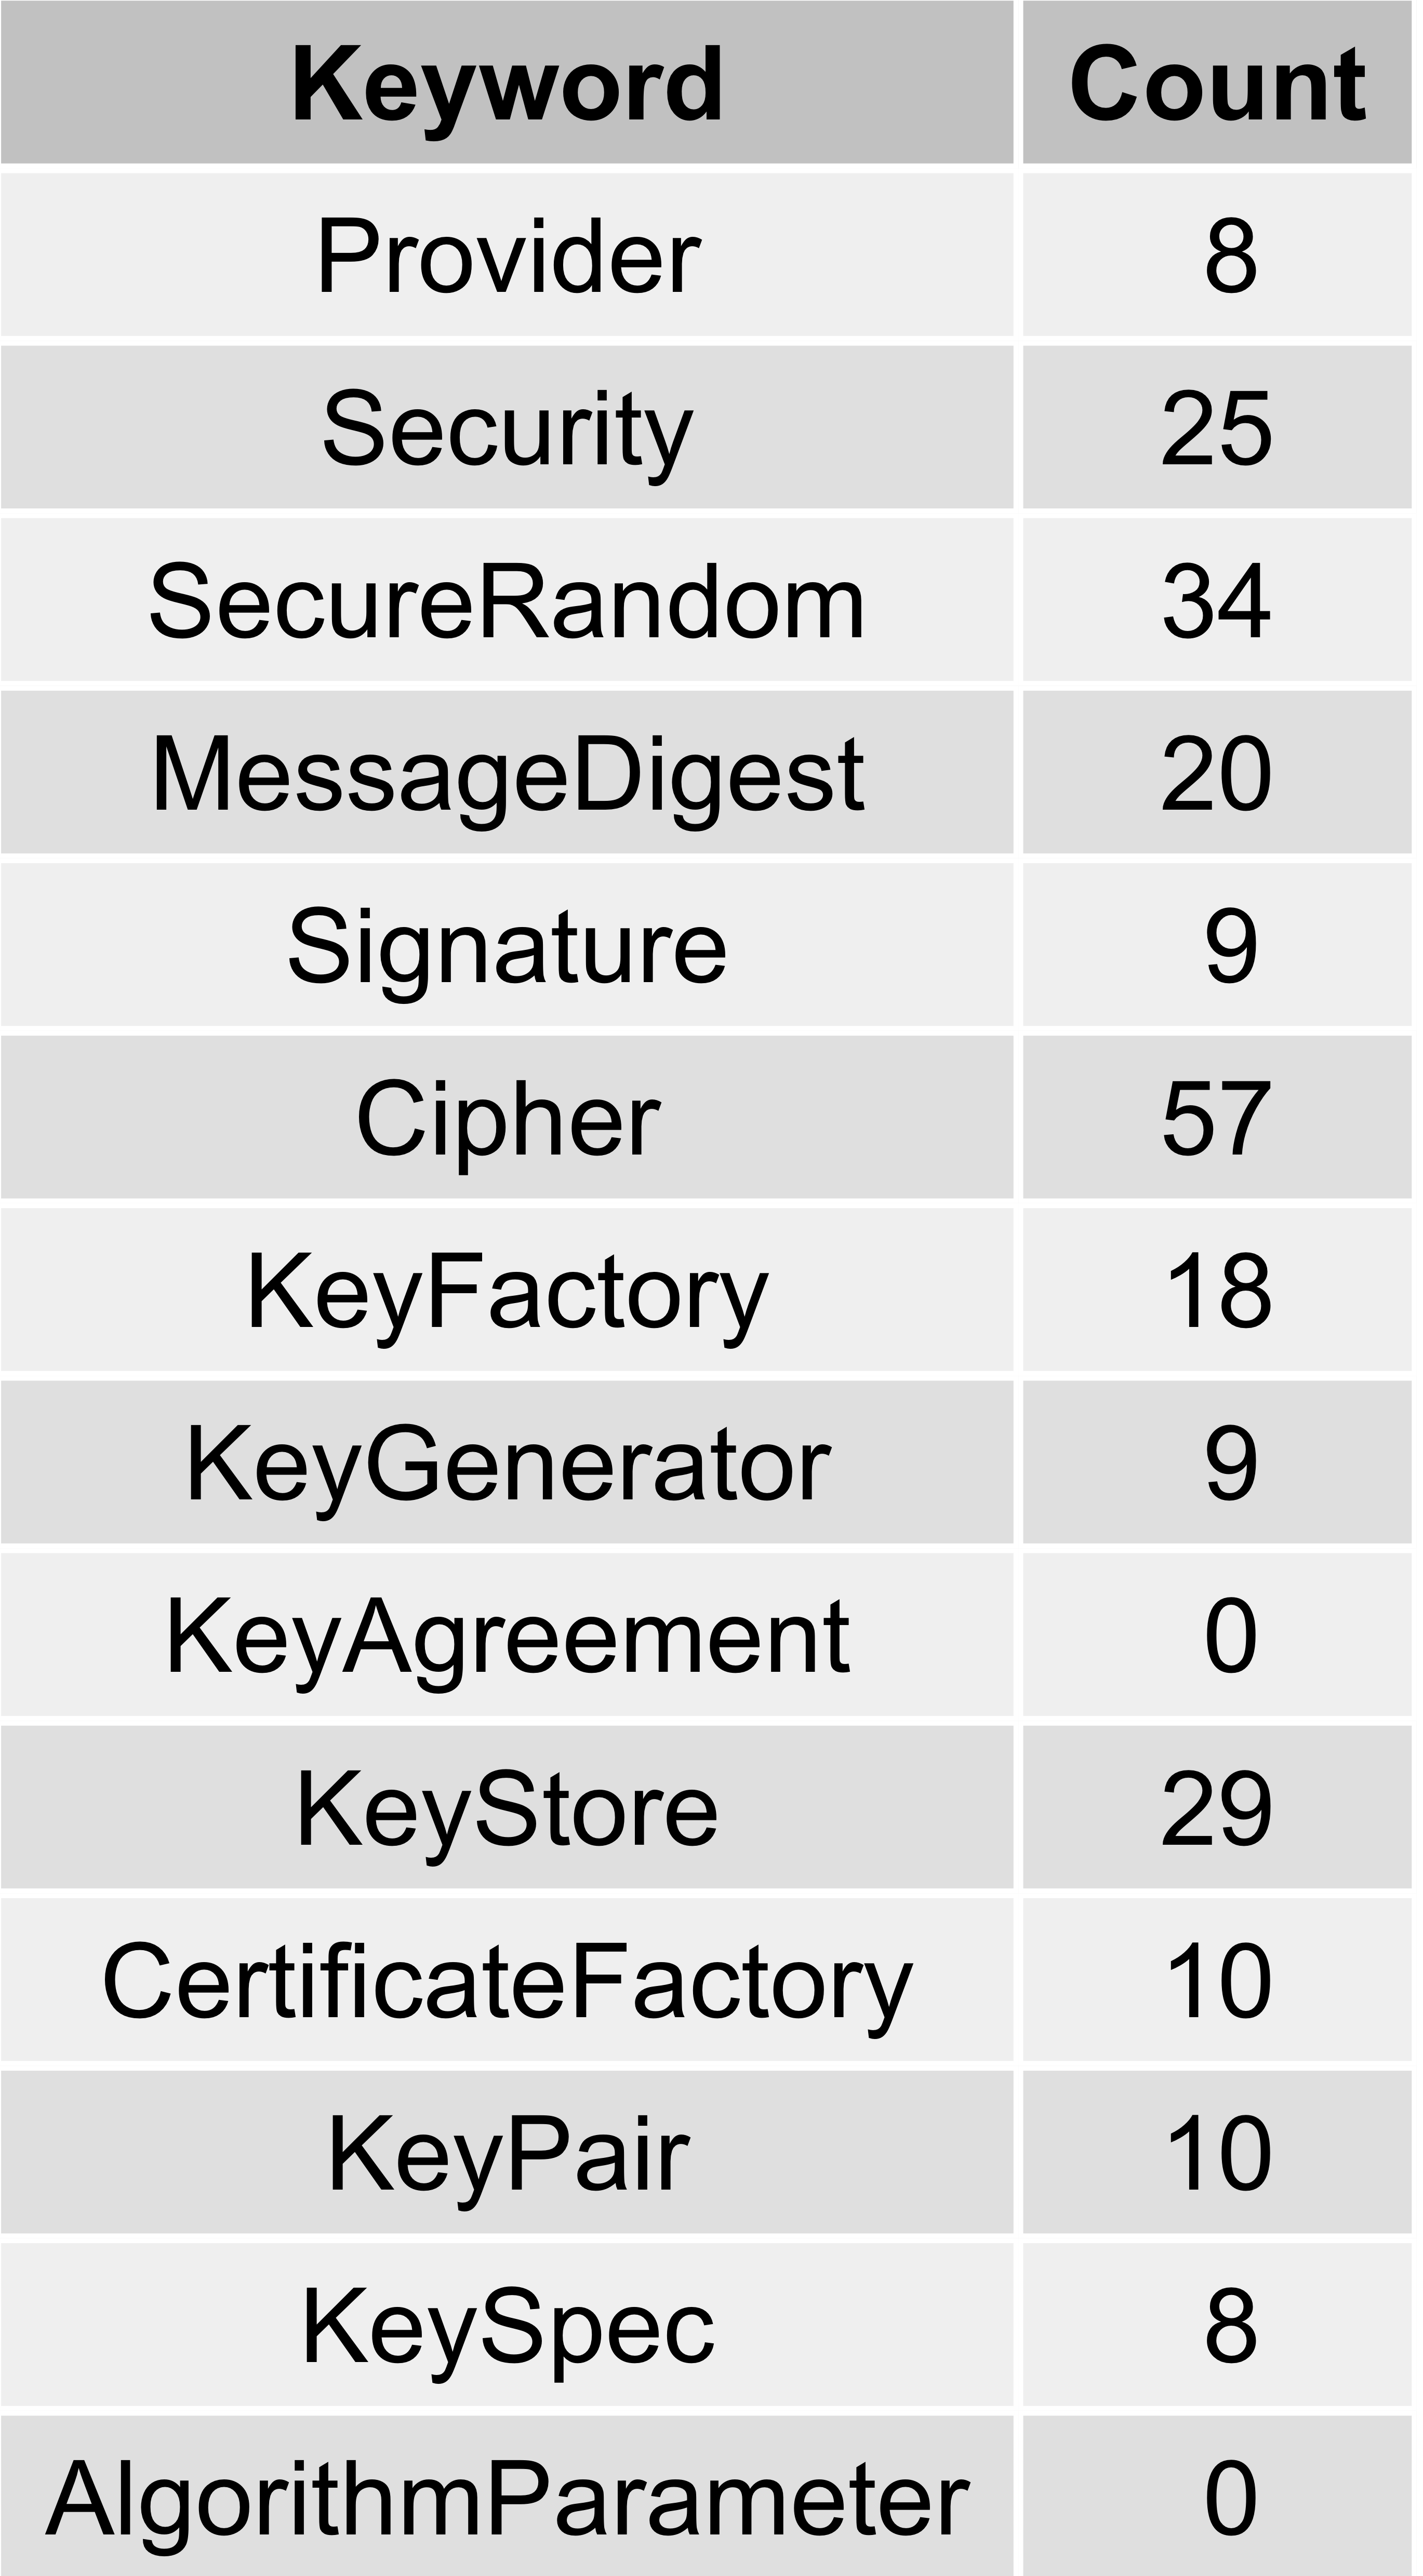
\includegraphics[width=0.5\linewidth]{KeywordCounts.png}
\caption{Counts of Snippets Containing Each Keyword}
\end{center}
\end{table}

These keywords were chosen as they are listed by in the JCA documentation \cite{JCA} as the core classes and interfaces of the JCA.

Admittedly this search was performed over the entire content of the snippet and as such may result in false positive cases. For example a code snippet that contains a comment mentioning one of the classes, but not actually using it will be included in our data sample. A possible remedy to this would have been to remove comments from snippets as a preprocessing step. 


We also evaluate two variants of technique for searching for keywords. The first technique accepted the keywords as matching in any portion of a string. For example SecurityManager would match on the keyword Security. This approach is a bit generous though, and potentially not necessary for the collection process. The reason that we initially considered this approach is that it may be better to attempt to process more snippets than necessary, in a batch processing style, so that it is less likely that we miss some relevant data. However upon second thought it appears that this approach will have no added benefit over a search that disallows matches on adjacent alphanumeric characters, but accepts symbols. For example SecurityManager would not match on the keyword Security, but Security.setProperty("someproperty") will match. We believe that this technique is more realistic for modelling the possible usages of class identifiers in Java, however we maintain the results of both strategies throughout the rest of the results for comparison purposes. 
From this point we will refer to the first strategy as partial match, and pure match.

The counts presented in Table 1 have been obtained as the pure match total of each from the entire set of snippets, as a result it is certainly possible for one snippet to include multiple keywords. As a result of this these counts may not necessarily give us a complete idea of the distribution of topics in posts, however we can potentially view the discrepancy in counts as interesting nonetheless. For example from the distribution we can see that it appears that more people are posting about Cipher, KeyStore SecureRandom, and, MessageDigest, as opposed to KeyAgreement and AlgorithmParameter. This makes a lot of sense, since, as listed on the JCA website, the "most useful high-level classes" include Cipher and MessageDigest. Classes such as AlgorithmParameter are moreso a support class for classes such as Cipher, so it is perhaps the case that they are more straightforward to use and therefore there will not be as many code snippets demonstrating the usage of these classes.
 

One issue here that we considered is that the names of methods and objects in a partial program are only identified by partially quantified names (PQN). A complete program will have full quantified names (FQN) for objects at the compilation step. The problem here is that there logically cannot be a constraint on Java as a programming language that would prevent multiple classes from different packages from having the same name, and in fact that is completely unnecessary, as a FQN is unique. The problem only arises when we are not provided information about the provider of a class (recall that only 6\% of the snippets had an import). One example of this can be seen in javax.ws.rs.ext.Provider and java.security.Provider. Both classnames are Provider, however they are clearly provided by different packages and have different functionality. The java.security.Provider implementation "represents a "provider" for the Java Security API" \cite{Security.Provider}, while the javax.ws.rs.ext.Provider is an implementation of "providers are application components that allow for customization of runtime behavior in three key areas: data binding, exception mapping, and context resolution" \cite{jax.Provider}. Thus these classes must be handled as unique. 

This particular example actually was observed in our data sample. Our search for keyword terms would detect snippets using the javax.ws.rs.ext.Provider, because Provider.class is a valid use of that type, and we do not filter these snippets out specifically. However a manual analysis revealed that only 2 cases of snippets contained this type of Provider, instead of the java.security.Provider, and these 2 snippets did not proceed through the compilation stage.

Previous works \cite{Subramanian:2014:LAD:2568225.2568313} have investigated resolving PQN to FQN by using variants of oracles to determine which possible types the ambiguous class name or method name could actually resolve to. In many cases, given a concrete implementation of a standard library, it is easy to tell if a class name corresponds to a valid type in that library. 

When it is the case that there could be multiple resolutions, it would be semantically incorrect to treat the object as any of those. This is highly relevant in our study since CogniCrypt's ruleset is defined over specific types, and an attempt to apply those rules to a "similarly" named but semantically inequivalent implementation would ruin the foundations of the analysis.

Luckily Soot PPA handles this for us,in a way it is our oracle. It works to perform type recovery when it can, and in the case that a type is ambiguous and cannot be recovered, it makes a safe approximation of that object by classifying it as unknown. This is completely safe, as then the object is still modelled loosely in the bytecode representation of the snippet, but CogniCrypt obviously does not have any rules for unknown objects and therefore will not report them as the source of violations of rules.

\section{Evaluation}

\subsection{Compilation of Snippets Using Soot PPA}

As previously mentioned we had to deal with the constraint that the snippets needed to be compiled. One previous work that used WALA to perform analysis \cite{7958574} actually cites using Soot PPA integrated into WALA to perform an analysis at the IR level. However they do not mention explicitly dealing with any of the Java version limitations that we encountered, despite the study being performed in 2017. They, and others \cite{Subramanian:2013:MSO:2487085.2487106} adding missing class and method declarations to the snippets. We perform this step, as well as a few other tweaks, guaranteed to not compromise the semantics of the snippets. In each iteration of compile attempts we perform the same tweaks. 

For each iteration we additionally prepare the snippet with the same set of imports, which are necessary to complete compilation. The imports that we used are listed here. As we can see they are mainly related to standard library functionality (the util library), and also the JCA (javax.crypto ect). 

\begin{lstlisting}[language=java]
import javax.net.ssl.*;                                                                        
import java.util.*;                                                                                     
import java.lang.*;                                                                                     
import java.io.*;                                                                                       
import java.security.*;                                                                                 
import java.net.*;                                                                                      
import javax.crypto.*;
import javax.crypto.spec.*;
import javax.crypto.interfaces.*;
import java.math.BigInteger;                                                                            
import java.nio.charset.StandardCharsets;                                                               
import groovy.grape.Grape;                                                                              
import org.apache.shiro.crypto.hash.Sha256Hash;                                                         
import org.spongycastle.util.io.pem.PemObject;                                                          
import javax.ejb.EJBAccessException;                                                                    
import java.lang.reflect.Method;
\end{lstlisting}


The levels of adjustment that we iterate over are:

\begin{itemize}
\item
None
\item
Class Wrap
\item
Class and Method Wrap
\end{itemize}

The logic behind this design is that some snippets do contain both class and method declarations, and therefore will compile at the None step. For snippets that contain just a method declaration, they will compile at the Class Wrap step. For snippets that contain no class or method declarations, adding both will be necessary.

The necessary tweaks that we perform for each is as follows:
\subsubsection{Annotations}
Java Annotations were introduced in Java 1.5. For the purpose of this study we remove all snippet lines that contain a Java annotation. 

\subsubsection{Generics}
Java Generics were also introduced in Java 1.5. The purpose of generics is to transform runtime type errors into compile time type errors, thus aiding in type saftey. They are used to annotate what type is expected by certain methods. However removing just the annotation is equally syntactically correct, and will also compile (we don't address how this affects runtime type errors, as it is not necessary here). Therefore all generic annotations are removed from snippet lines that contain them.

\subsubsection{Preexisting Imports and Package Declarations}
10\% of snippets out those containing a keyword, and  4\% of snippets contained a package declaration. We remove both pre-existing imports and package declarations. This is because for iterations 2 and 3 (class wrap and class/method wrap) a naive attempt to add these declarations to the file would place the declaration overtop of the imports or package declaration. This obviously would always yield code that would not compile. Package declarations are completely unnecessary to us here, and in order to assess the effect of removing pre-existing imports we extracted the set of pre-existing imports and manually verified that we readded any that had previously been there, so that we do not lose any type information that was intended to be conveyed. 
One note here is that the following imports in our master list were obtained from this step:
\begin{lstlisting}[language=java]
import java.math.BigInteger;                                                                            
import java.nio.charset.StandardCharsets;                                                               
import groovy.grape.Grape;                                                                              
import org.apache.shiro.crypto.hash.Sha256Hash;                                                         
import org.spongycastle.util.io.pem.PemObject;                                                          
import javax.ejb.EJBAccessException;                                                                    
import java.lang.reflect.Method;
\end{lstlisting}
This is fine for Soot PPA, however if attempting to use the javac compiler, the imports that are not from the standard java library will need to be removed again.


After assessing which snippets could not be successfully compiled, we were left with a sample of 173 snippets to run CogniCrypt on in the partial match condition, and 96 snippets to run CogniCrypt on in the pure match condition. 


\subsection{Comparison on Search Techniques}
Before discussing our interpretation of results, we first revist a slightly more empirical comparison of the two applied snippet search techniques. The following distributions are obtained by applying a pure match approach to collect a count of keywords existences in each snippet that has been compiled.

Now that we have fully described our technique for obtaining 
\begin{figure}[h]
\begin{center}
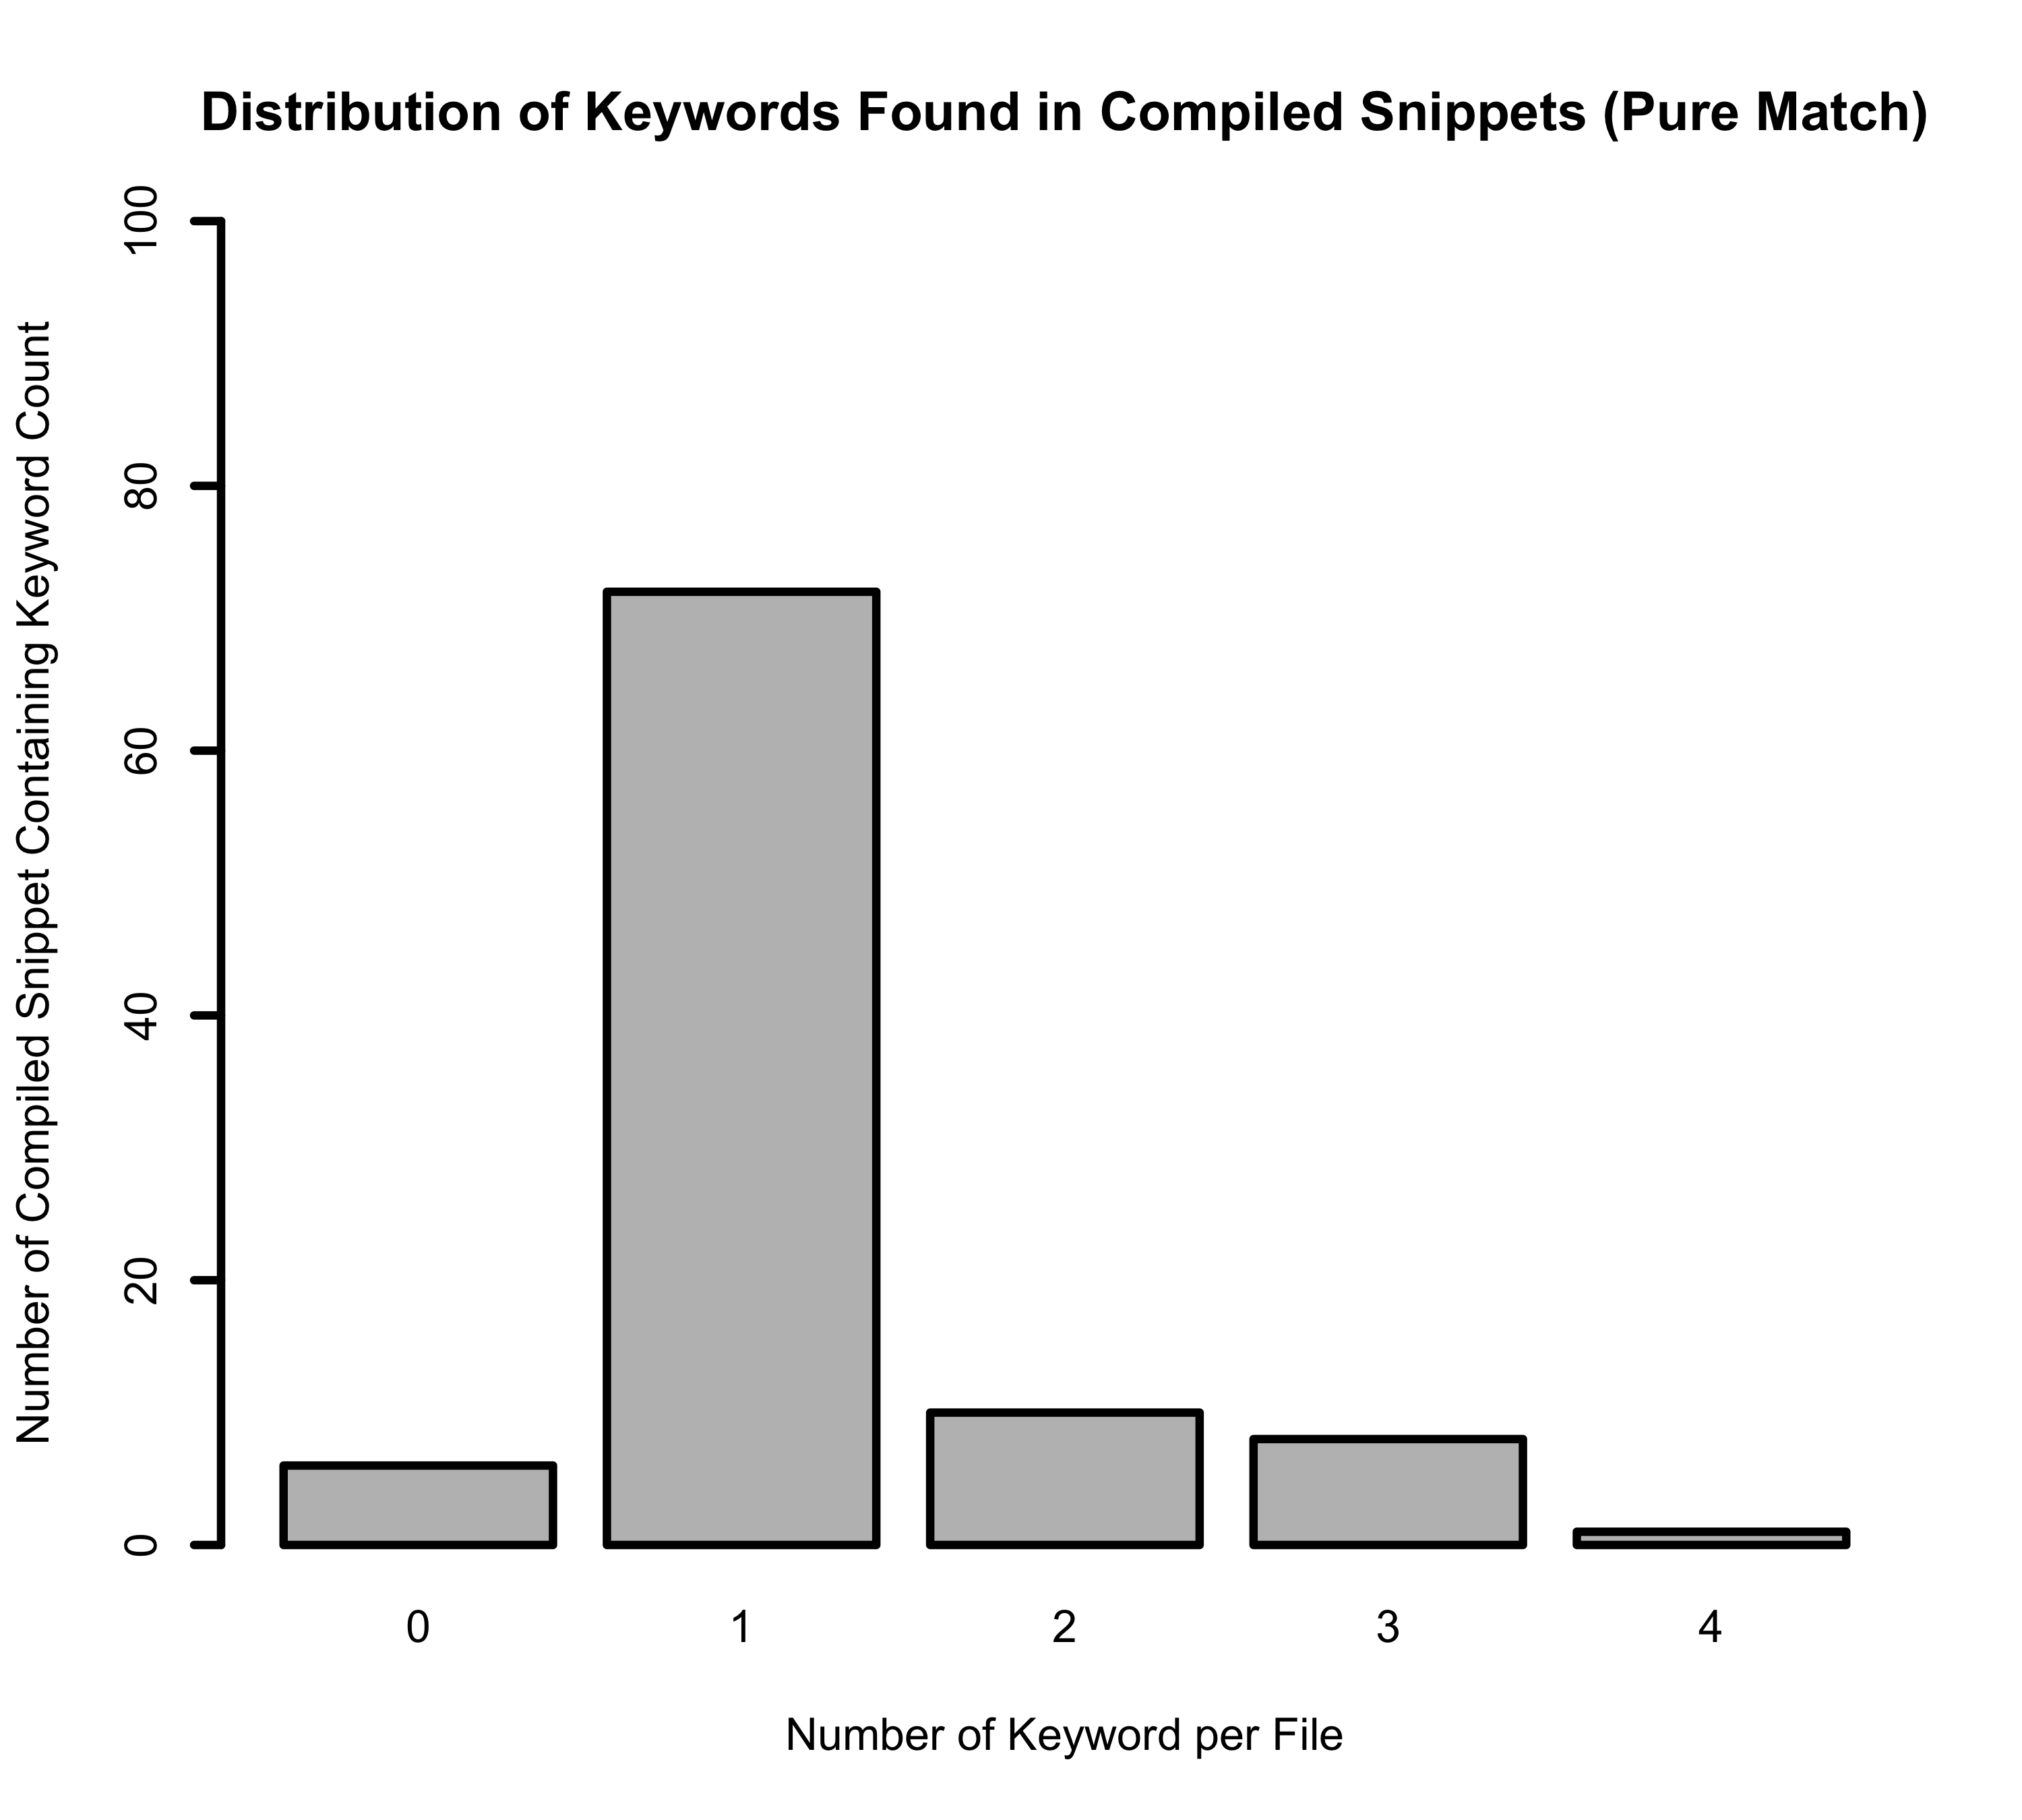
\includegraphics[width=0.9\linewidth]{CompiledKeywordDistPureMatch.png}
\caption{Counts of Keyword Matches in Compiled Snippets}
\end{center}
\end{figure}

\begin{figure}[h]
\begin{center}
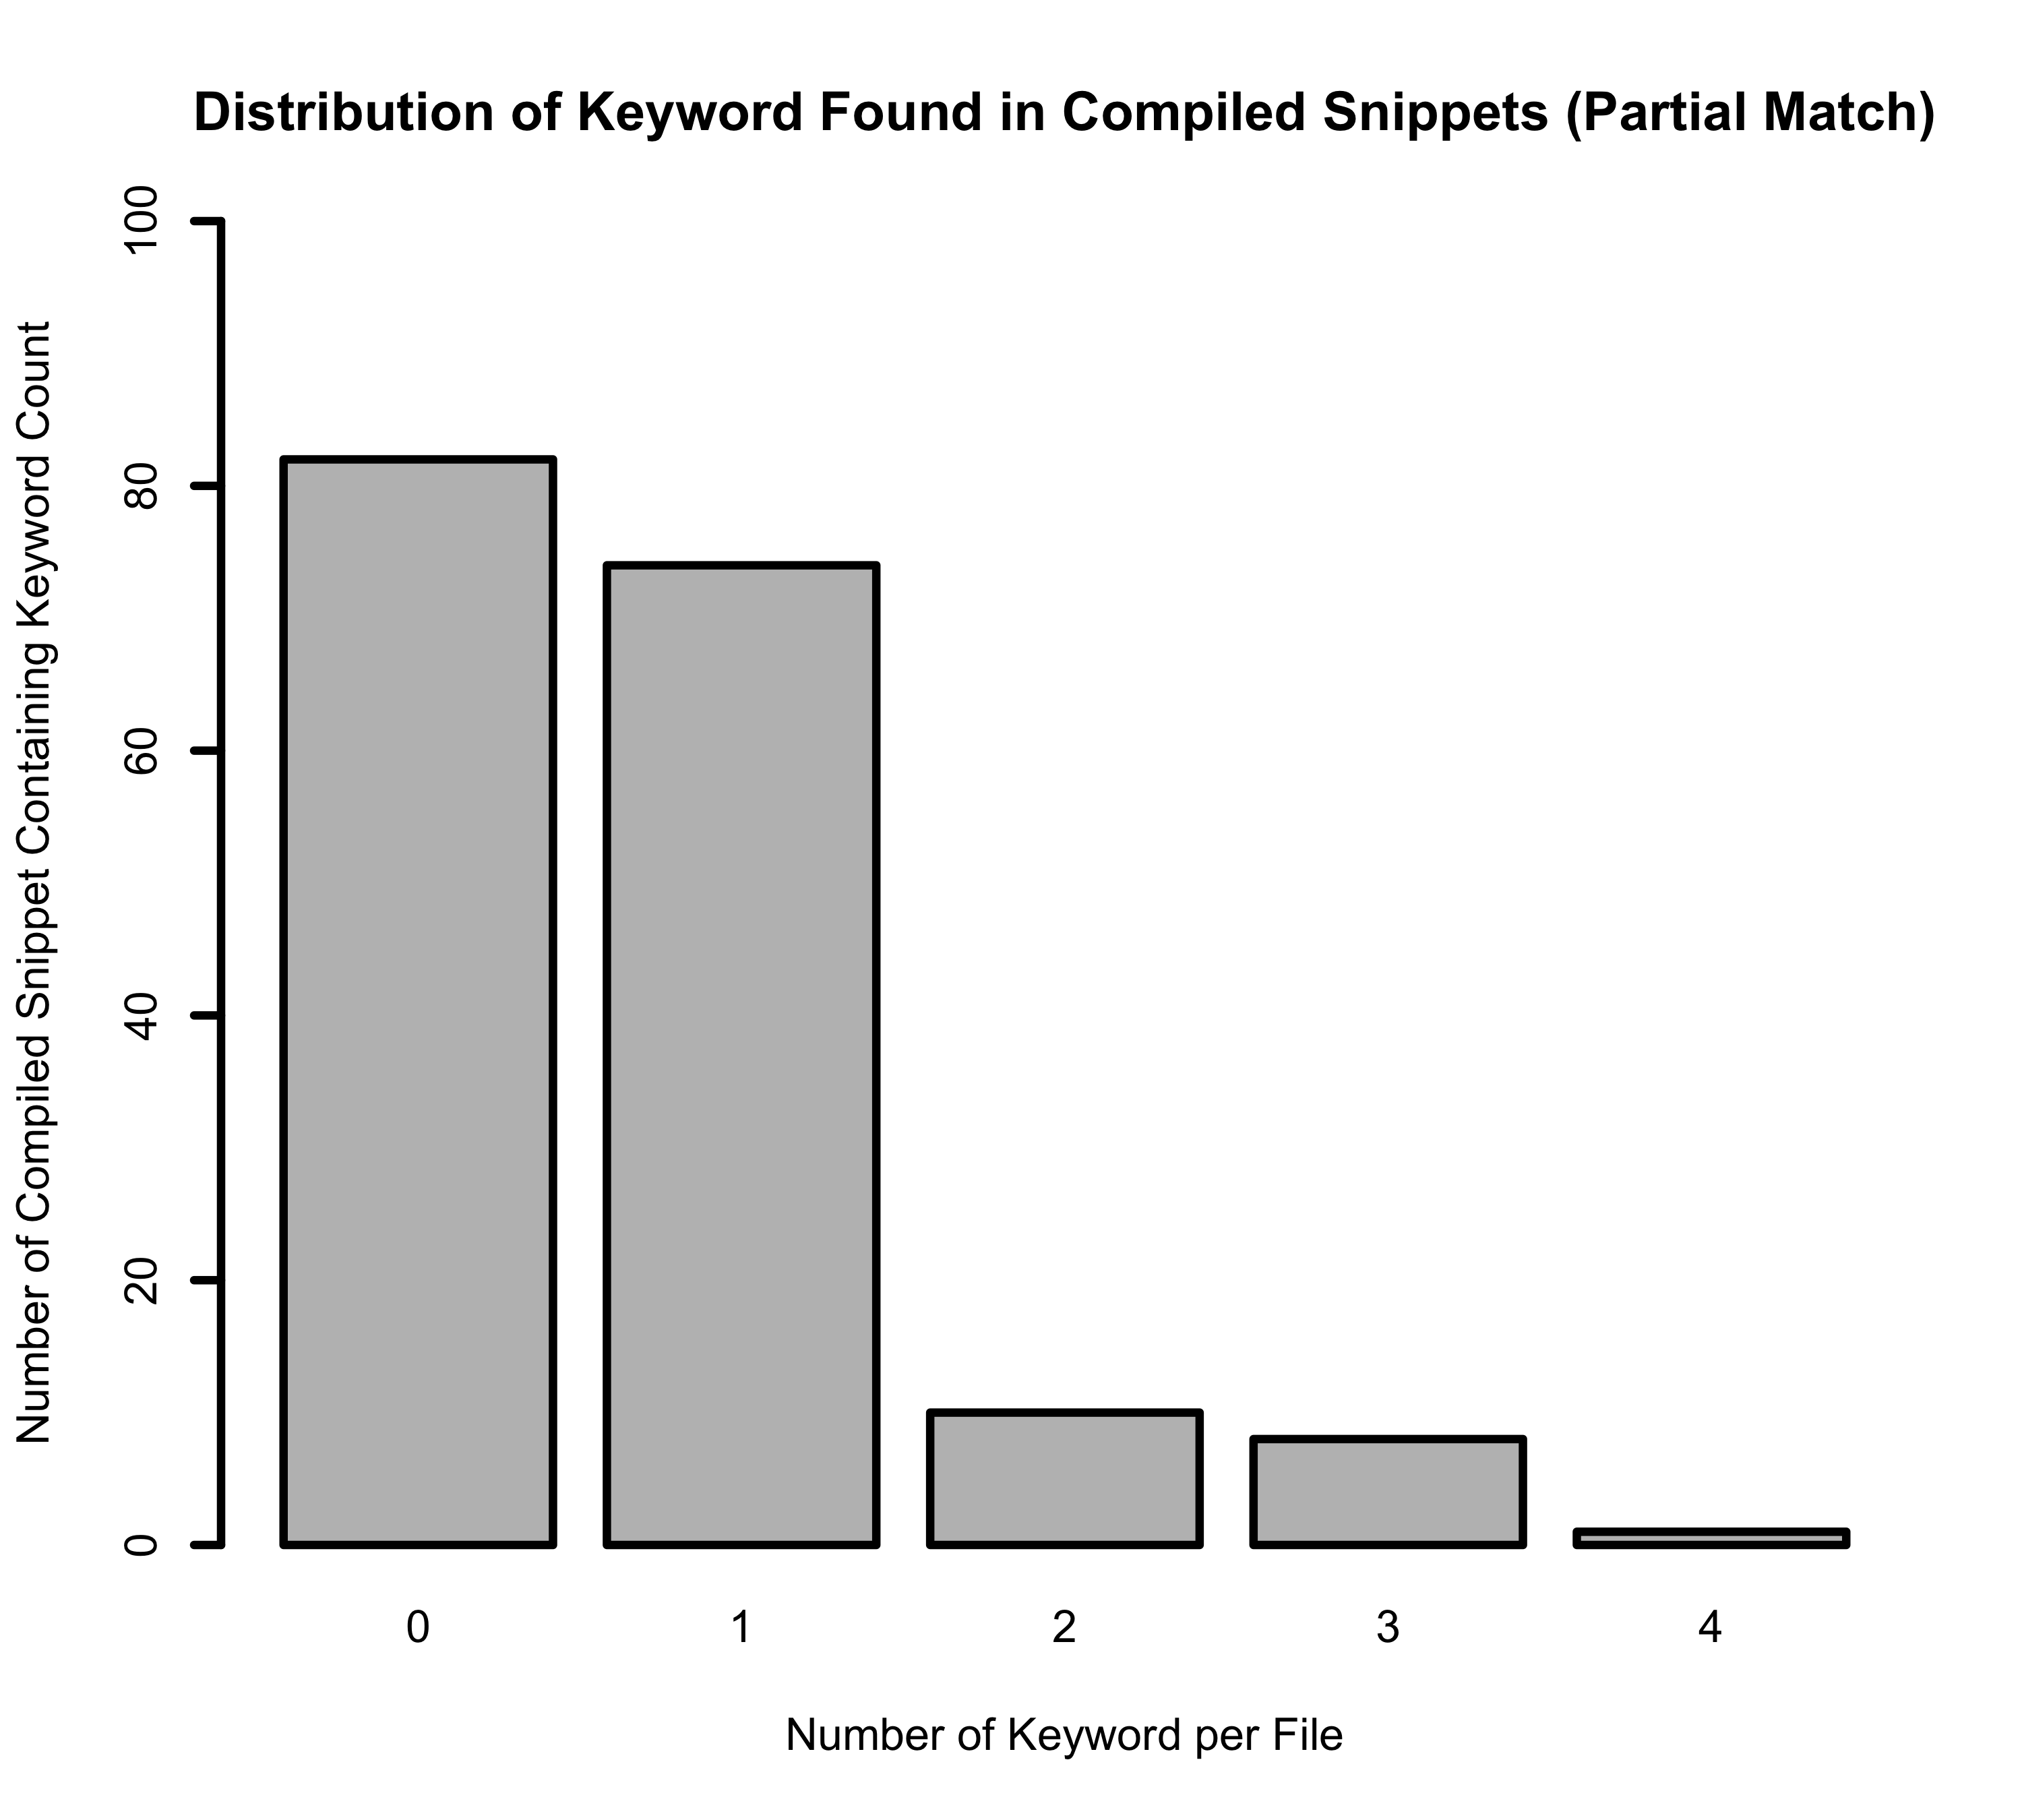
\includegraphics[width=0.9\linewidth]{CompiledKeywordDistPartialMatch.png}
\caption{Counts of Keyword Matches in Compiled Snippets}
\end{center}
\end{figure}

From these distributions we can see that pure match and partial match, not surprisingly find the same number of snippets containing one through four keywords. However the partial match technique detects 76 more snippets as relevant, however these snippets indeed have 0 keywords. It may also seem surprising to note that the pure match filtering condition can still yield snippets with no keywords once they are compiled. But if we consider the example listed earlier in our discussion of FQN/PQN, this actually makes sense. The example here was involving javax.ws.rs.ext.Provider is relevant because "Each JAX-RS provider class must be annotated with the @Provider annotation" \cite{jax.Provider}. However since Soot PPA cannot deal with Java annotations, as previously mentioned, these lines in the snippet will be removed in order to compile. Therefore even the pure match technique will inevitably yield an initial input set of snippets with no relevance to our pipeline process.

\subsection{Comparison Alternative Compilers}

\subsection{Javac}

The Javac compiler option could be considered as the ideal option of a compiler for our pipeline. This is because naturally the javac compiler has the sole goal of producing executable java bytecode. Unfortunately, unlike Soot PPA, which is conscientious to the goal of analysis, javac will halt upon all error types. It cannot resolve type ambiguities by assigning an unknown type, as that would disallow the JVM from knowing which class to load at runtime. We evaluate our pipeline with Javac substituted in place of Soot PPA and discuss the outcome below.

\subsection{Eclipse JDT}

We also evaluate our pipeline with Eclipse JDT substituted in place of Soot PPA and discuss below.

\section{Results}

\subsection{RQ1}

We discovered that we were indeed able to analyze some of the snippets and from these we did find a noteworthy number of cryptographic misuses. As previously discussed there are two significant barriers to analyzing the snippets. First the snippets must be compiled. Then they must have been compiled in such a way that they contain an analyzable object. That is to say they must be valuable to analyze. 

Lastly, we discuss the evaluation of our heuristic of relevant snippet selection. From Table 1 we have a total of 138 keywords occurring in our snippets. This should roughly correspond to the number of objects that we can analyze. However we were only able to find even one object to analyze in 19\% of the compiled snippets, and found a total of 59 objects that were analyzed across all of the snippets. 


In Figure 1 we can see that most snippets contained only one analyzed object. This makes sense, in that each snippet is demonstrating the functionality of only one object, and is not a complete demonstration of a complete piece of code. 
\begin{figure}[h]
\begin{center}
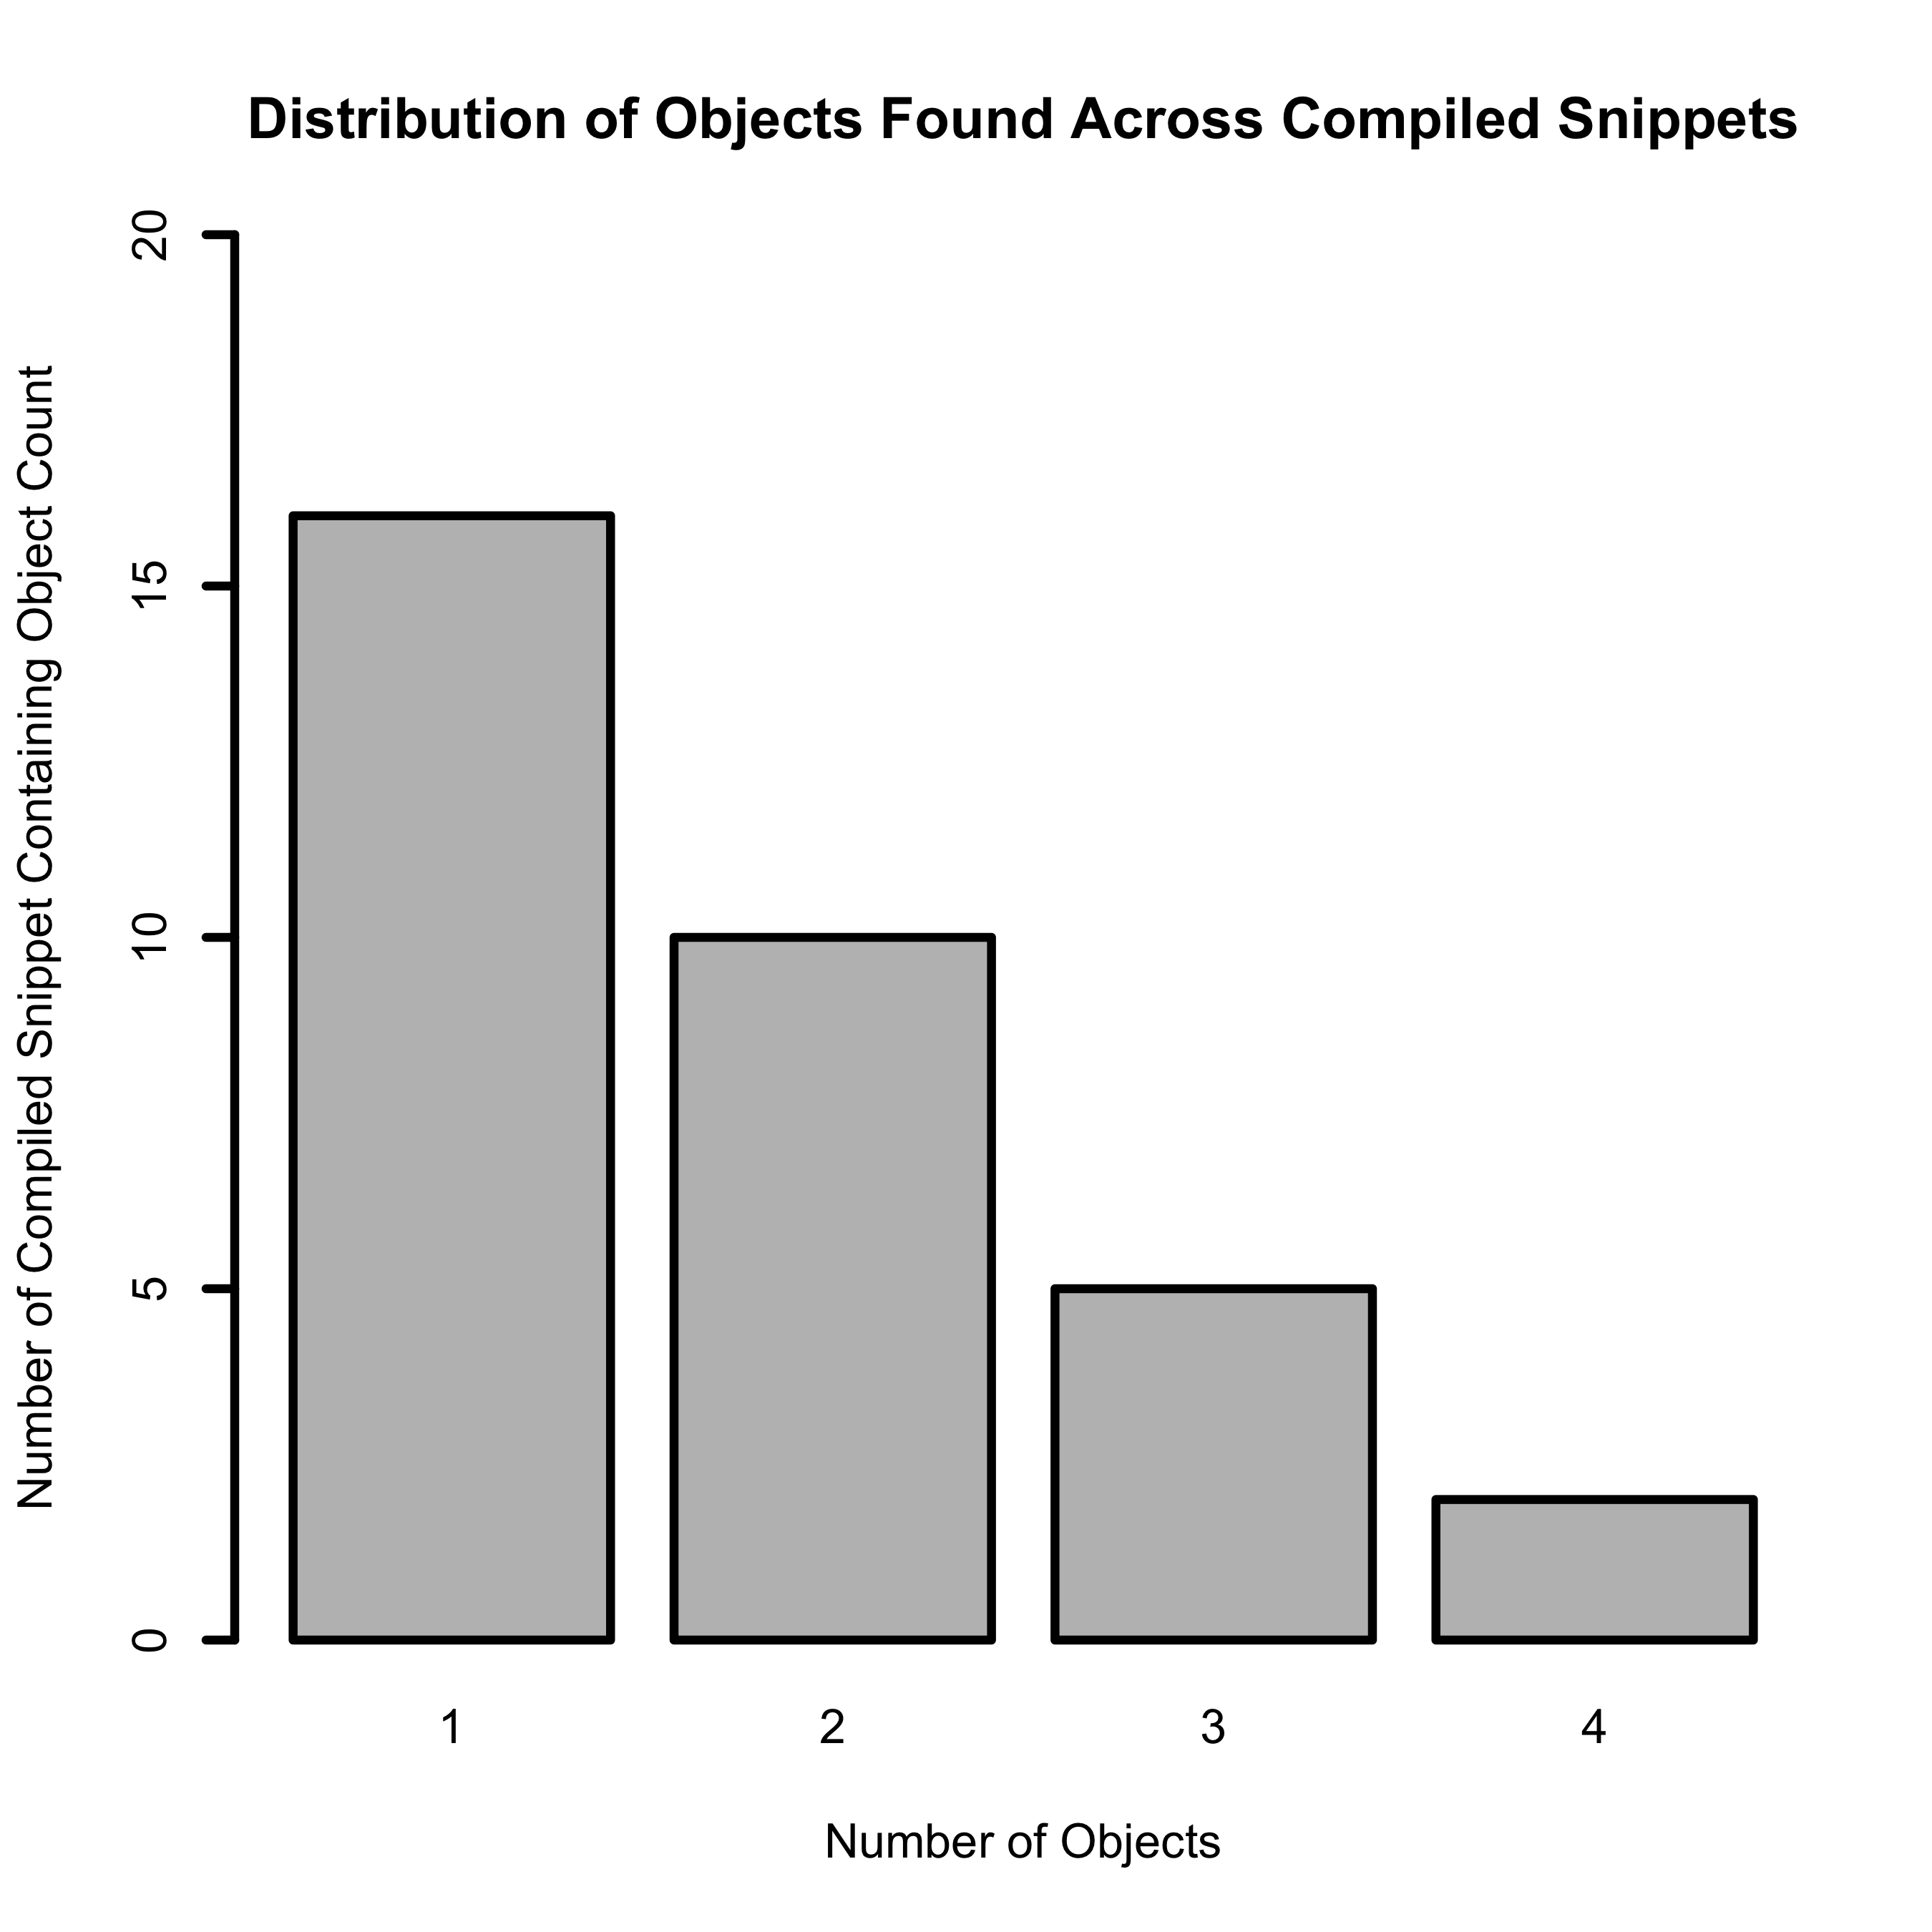
\includegraphics[width=0.9\linewidth]{ObjectDist.png}
\caption{Counts of Objects Analyzed in all Compiled Snippets}
\end{center}
\end{figure}

However if we compare this to the distribution of number of keywords in each snippet, as shown in Figure 2 we will see that . Our hypothesis for this discrepancy is that it arises from the type inference strategy of Soot PPA, and that it inherently cannot infer all types in incomplete programs, however a more thorough investigation would be required in order to conclude on this matter and ultimately improve the pipeline process described in this work. 

Lastly, as an anecdotal comparison point for our ability to compile snippets we would like to cite this work \cite{7958574}, where they were able to successfully process between 85 and 66\% of their sample. In this study they processed their sample to the IR level, and this may be one reason for the difference in success. As our results are not too drastically different we believe that it a roughly 50\% successful compilation rate is reasonable.

\begin{figure}[h]
\begin{center}
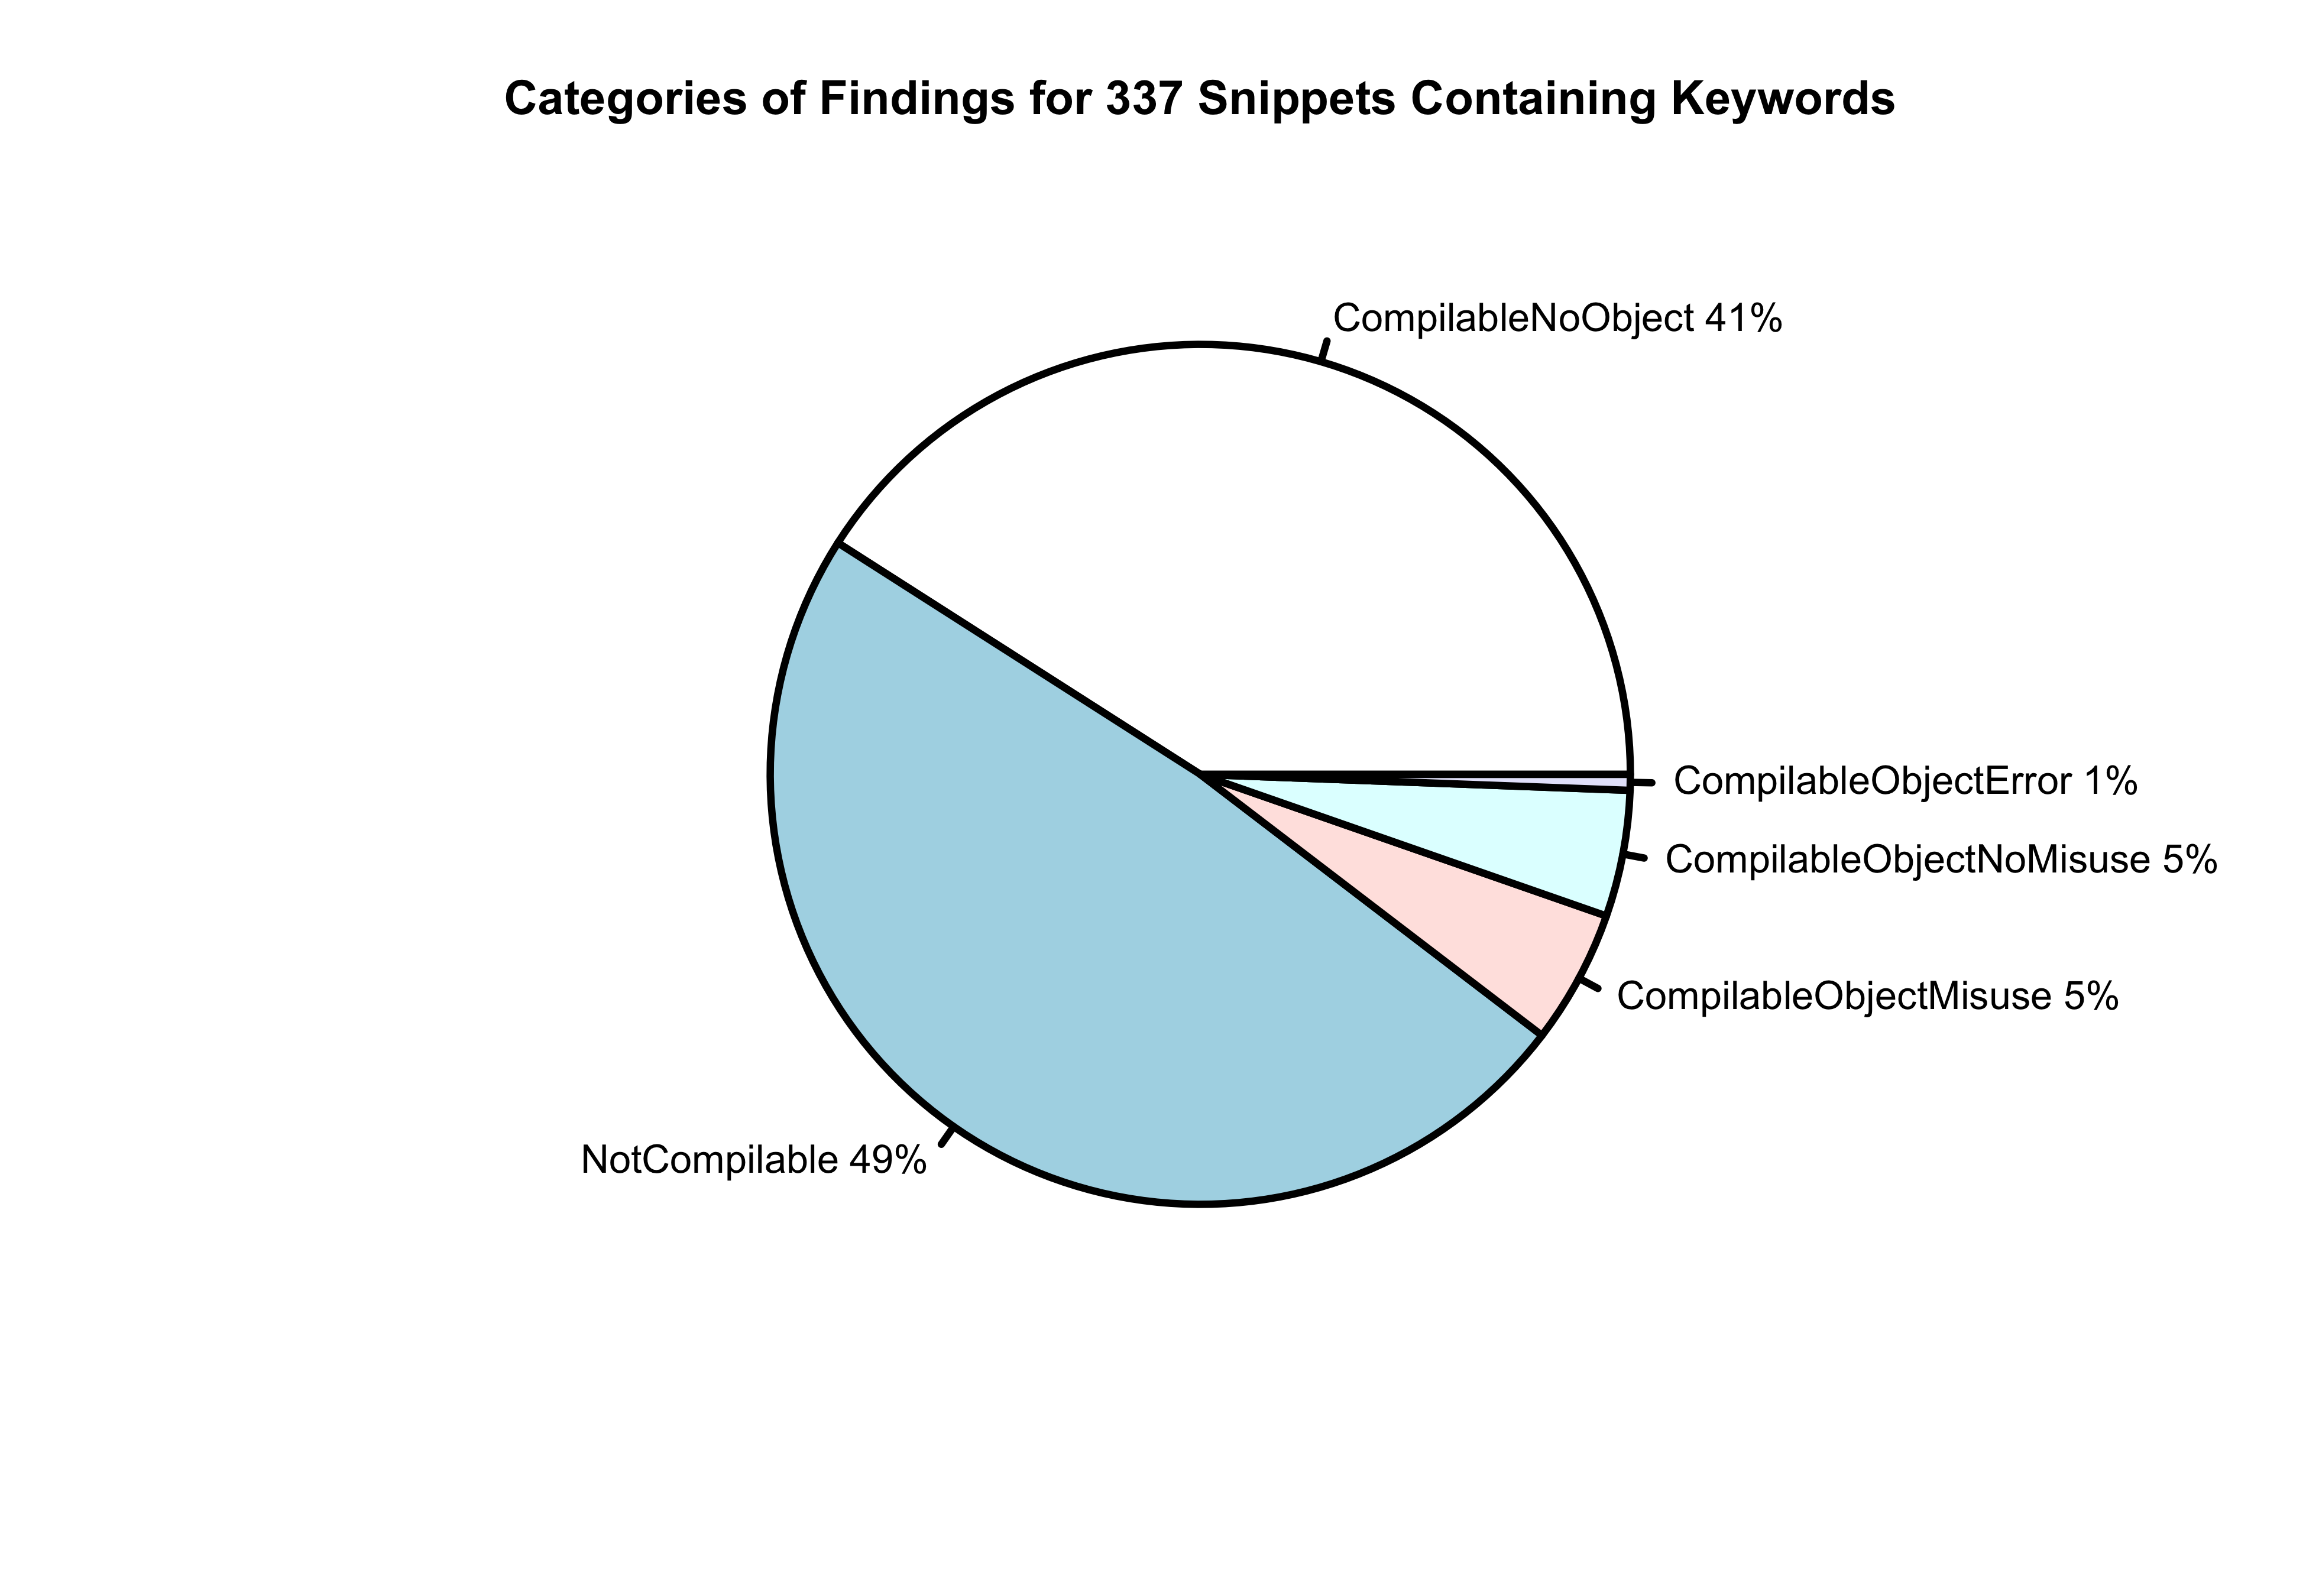
\includegraphics[width=0.9\linewidth]{PiePartialMatchFull.png}
\caption{Counts of Snippets at Each Level of Processing}
\end{center}
\end{figure}

\begin{figure}[h]
\begin{center}
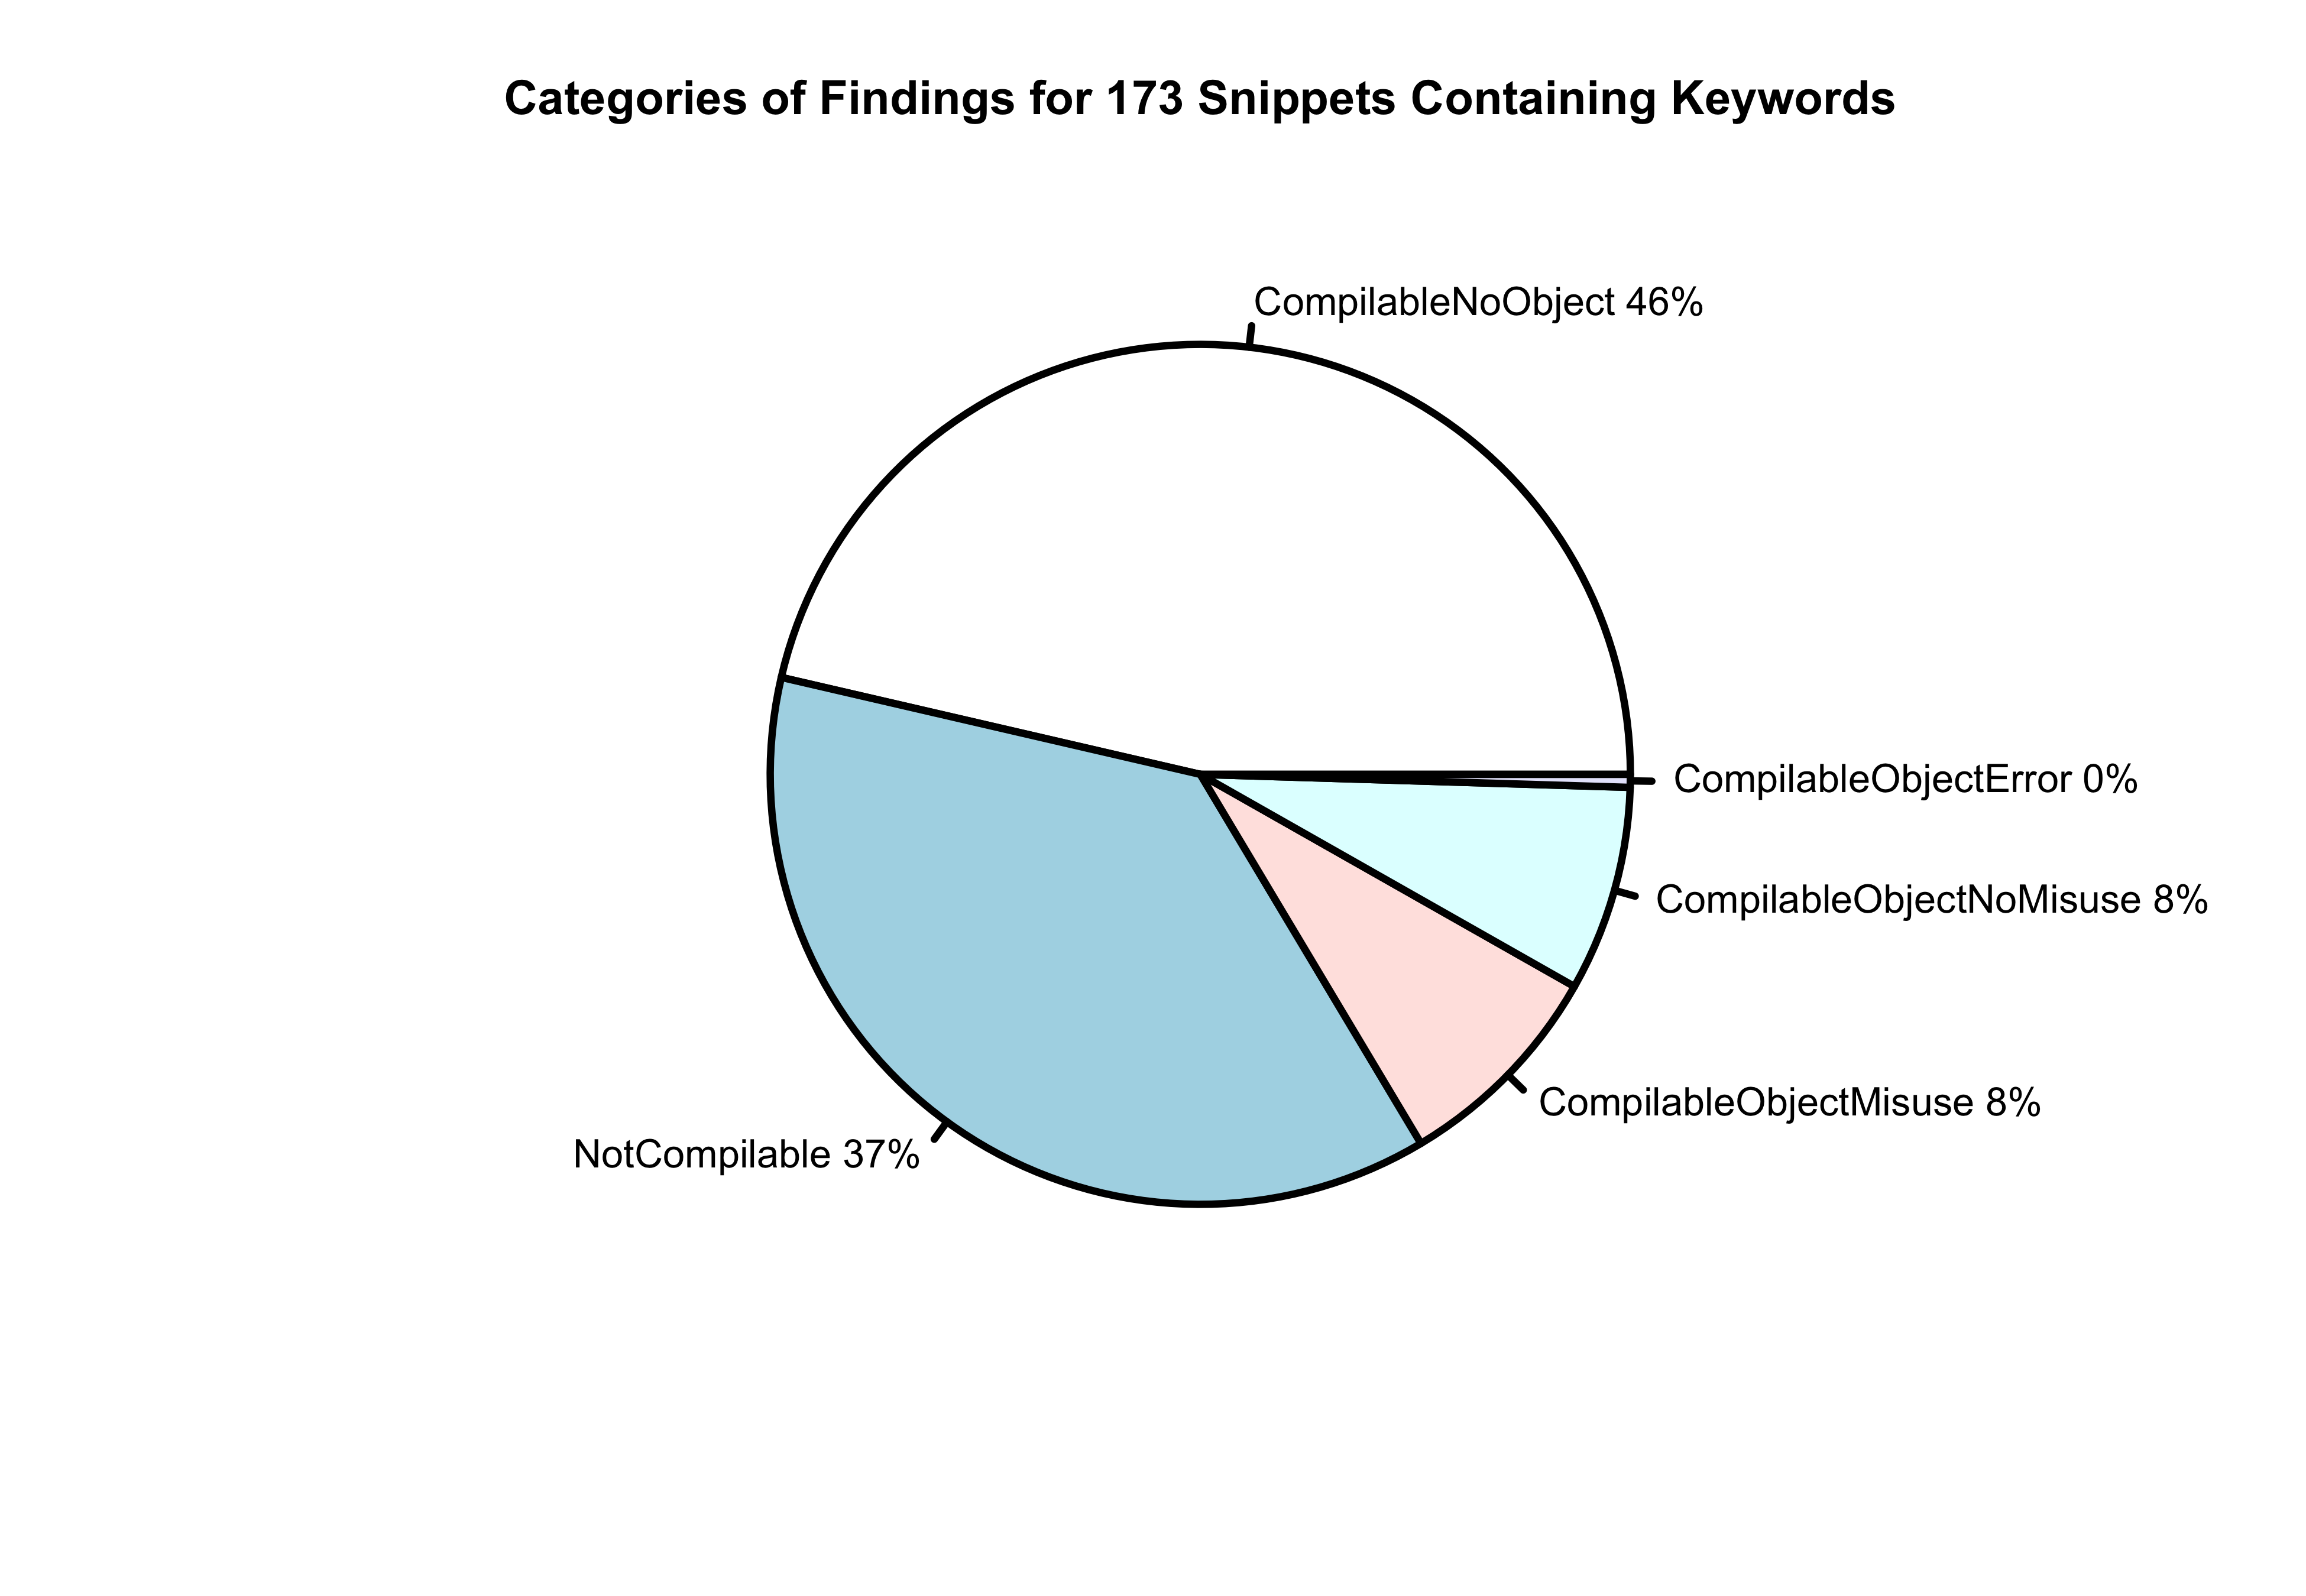
\includegraphics[width=1.0\linewidth]{PiePureMatchFull.png}
\caption{Counts of Snippets at Each Level of Processing}
\end{center}
\end{figure}

\begin{figure}[h]
\begin{center}
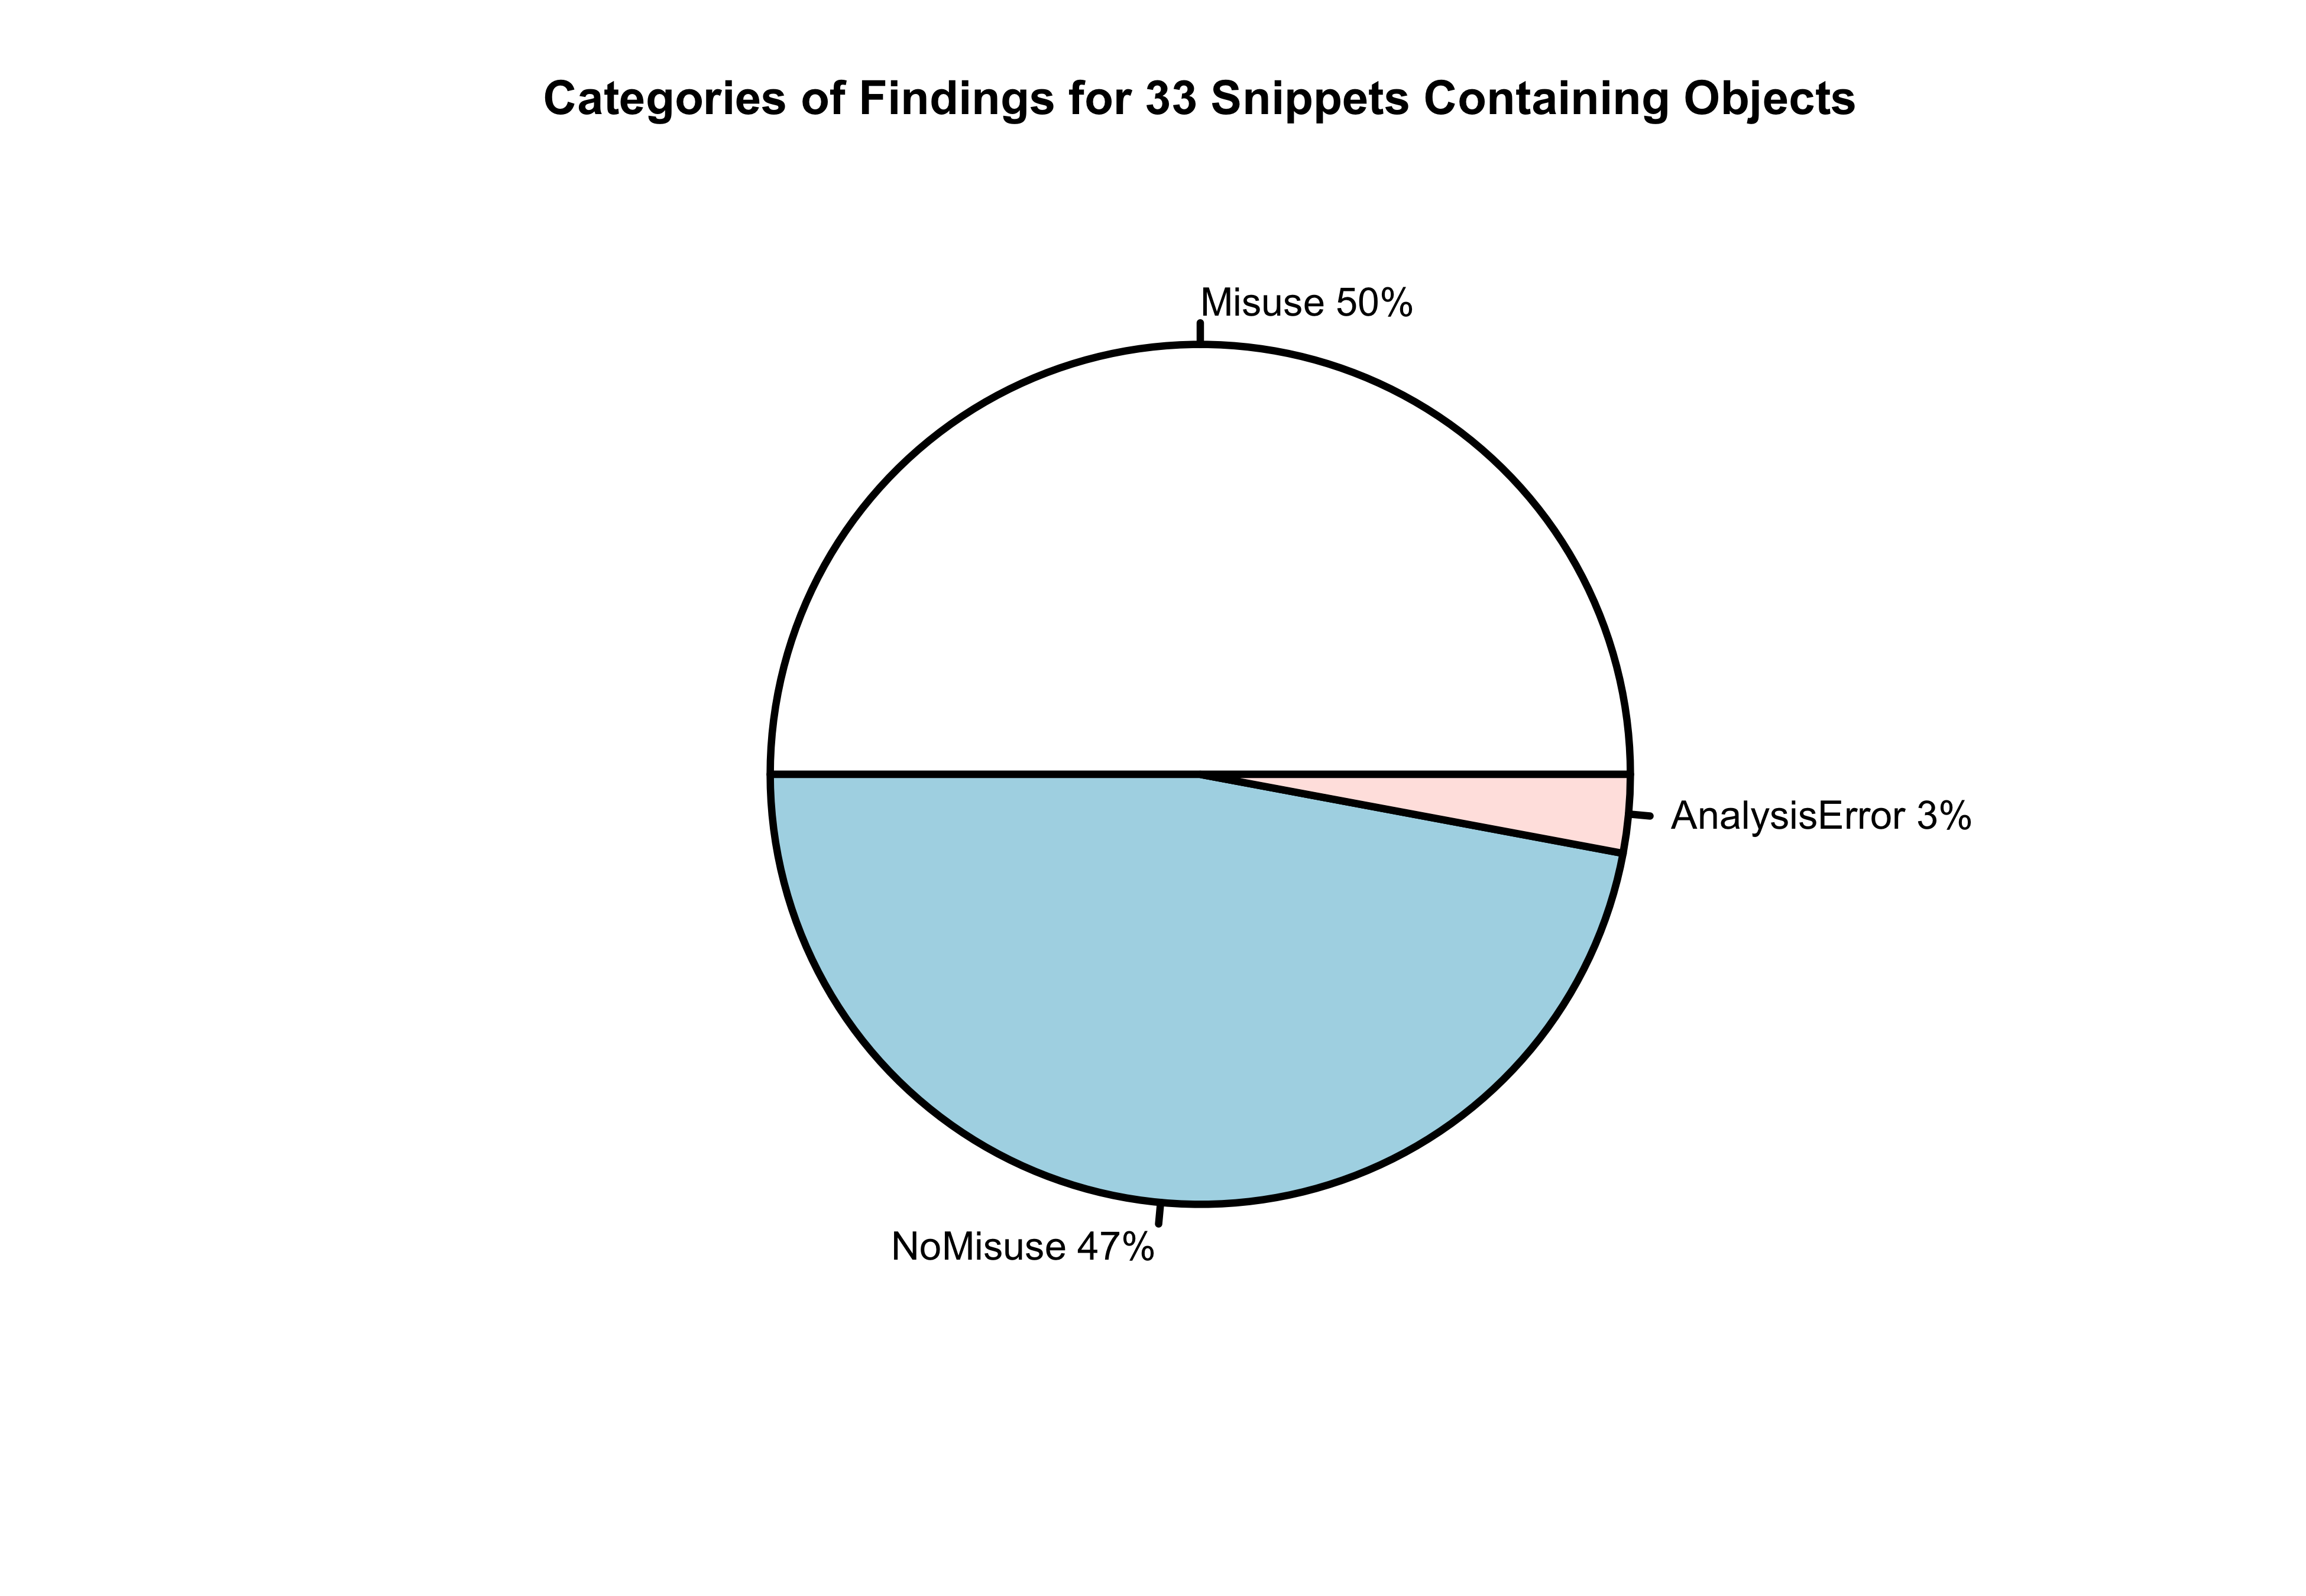
\includegraphics[width=0.9\linewidth]{PieObjOnly.png}
\caption{Counts of Snippets at Analysis Processing Phase}
\end{center}
\end{figure}


\subsection{RQ2}

The distribution of errors as reported by CogniCrypt is presented in Fig 2.

\begin{figure}[h]
\begin{center}
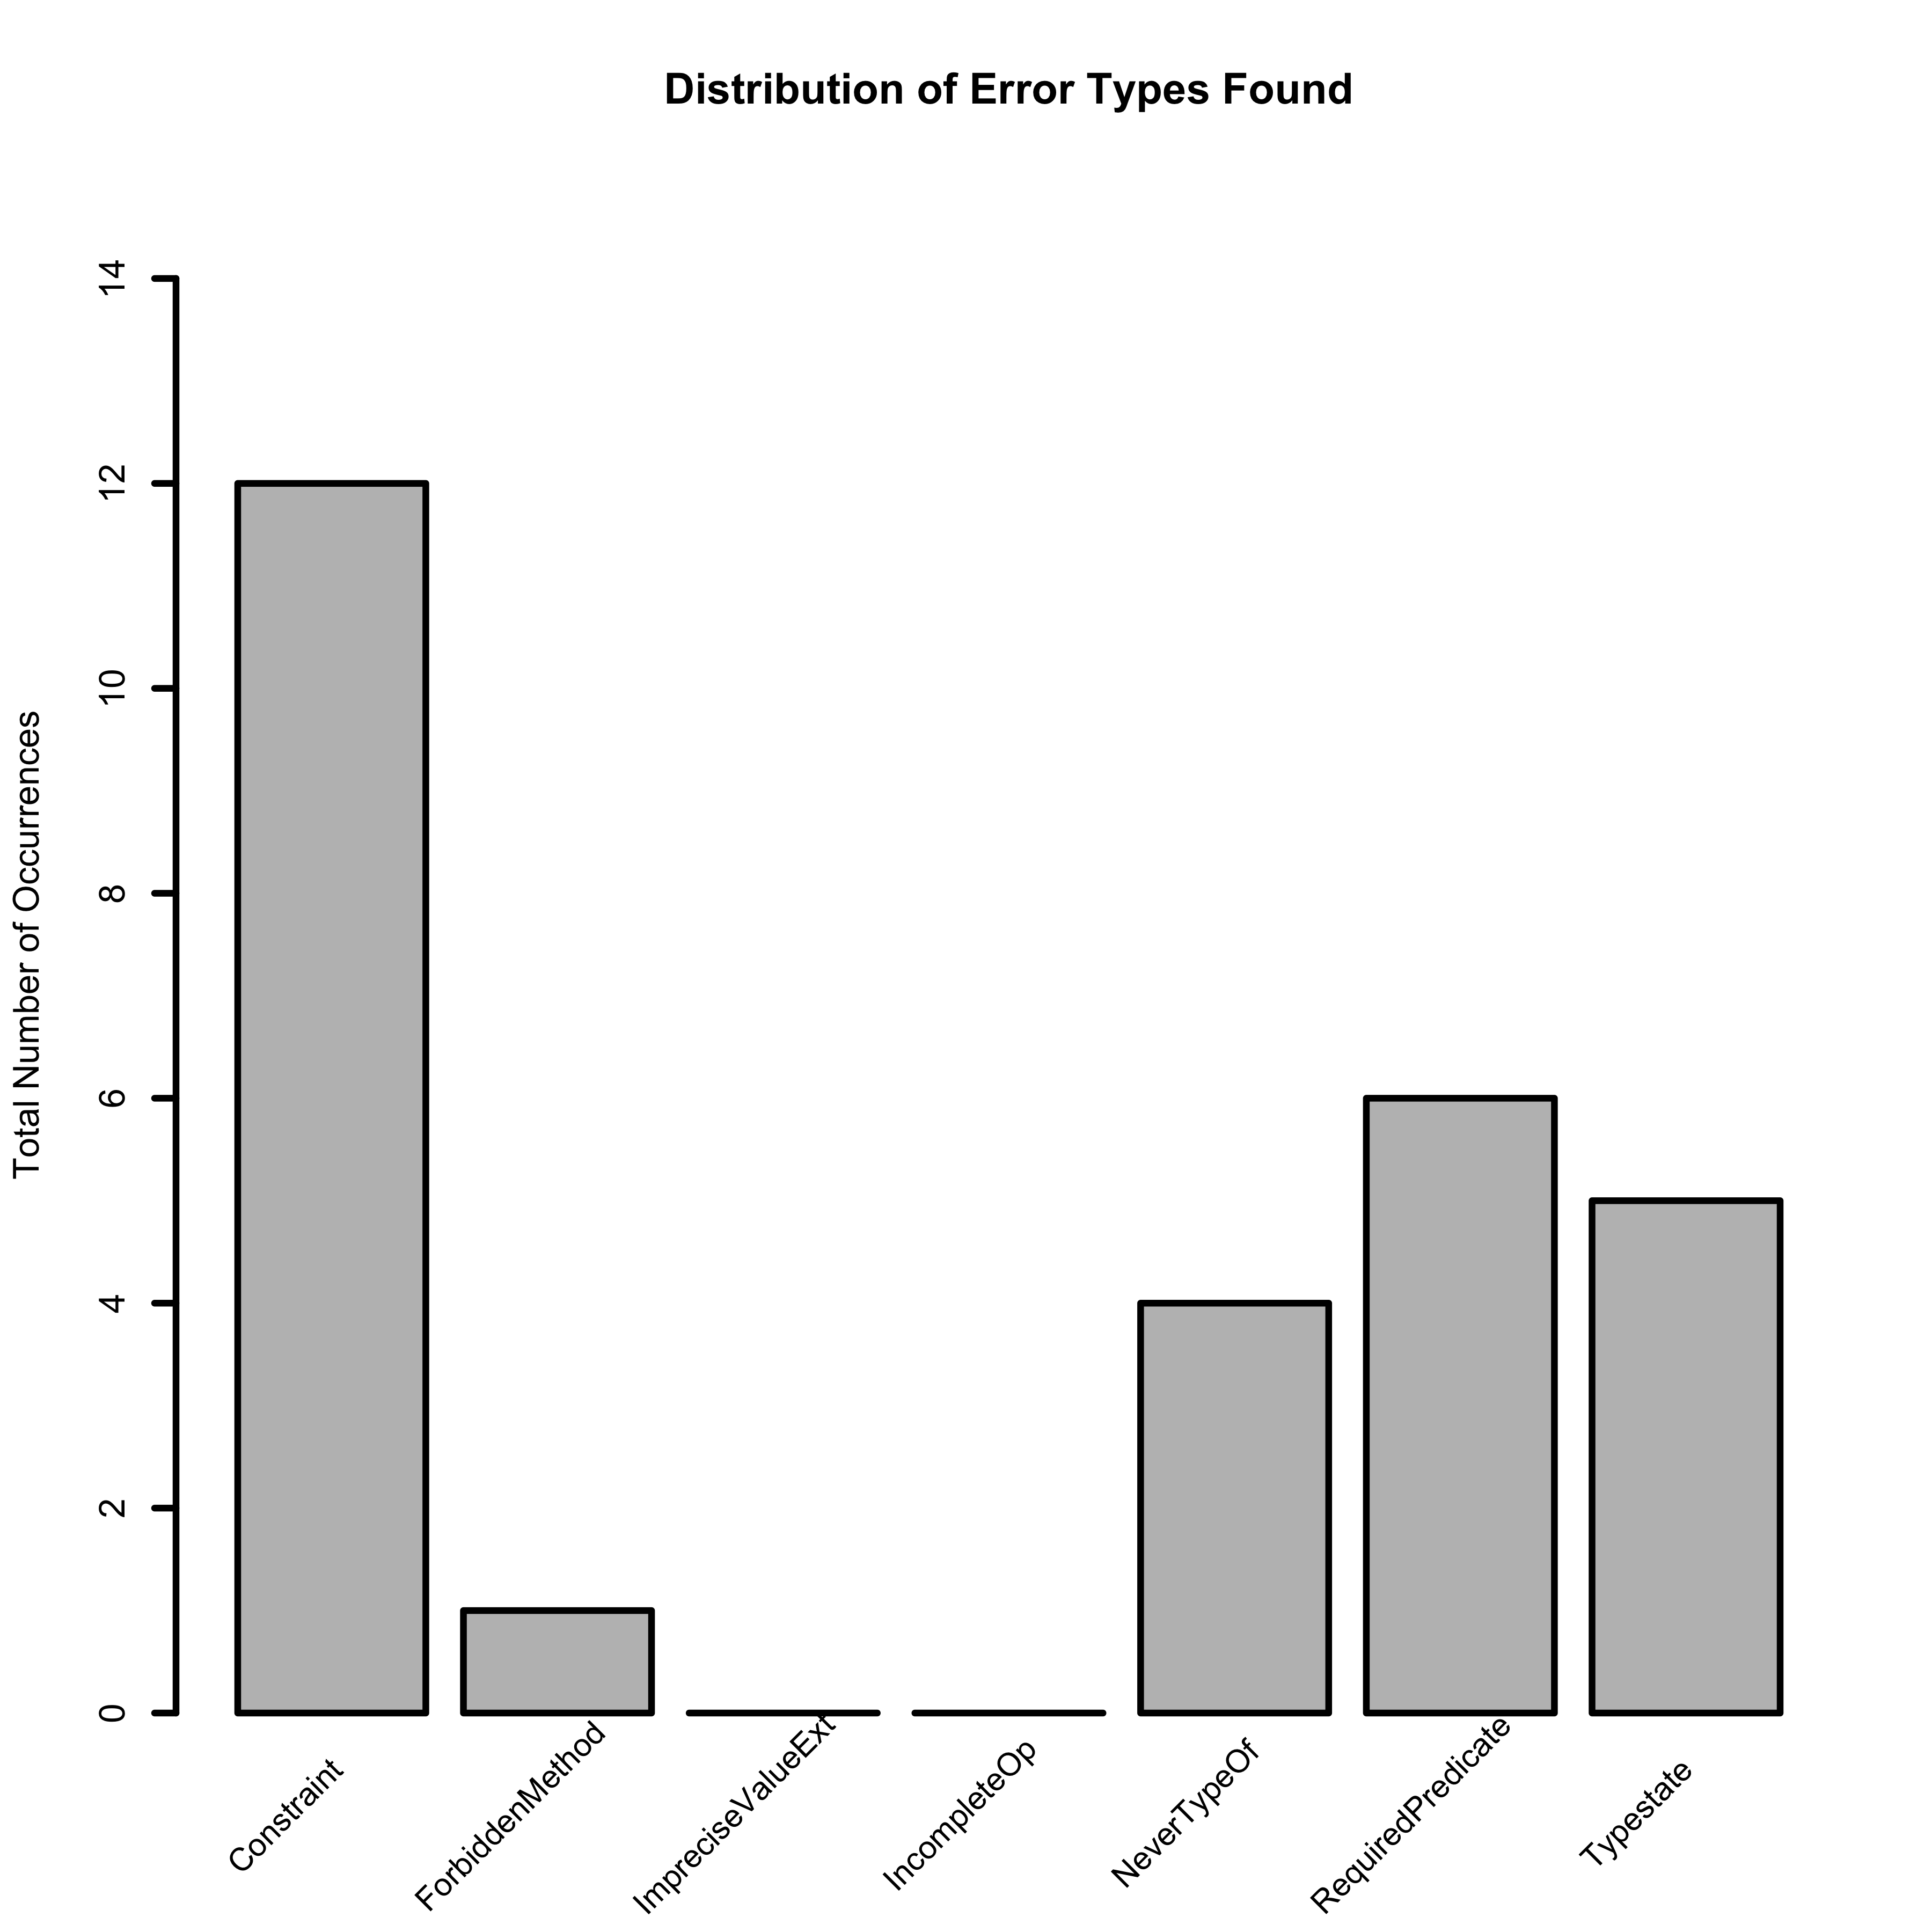
\includegraphics[width=0.9\linewidth]{Dist.png}
\caption{Error types generated by CogniCrypt}
\end{center}
\end{figure}

\subsection{RQ3}

In order to answer RQ3 we look at the number of GHUrls that correspond to unique projects that reference each SO post. 


\section{Discussion}

In light of the results that we have observed it is important to reconsider the big picture. In order to do this first we present an overview to the reader of the types of errors that CogniCrypt reports, so that we may discuss the implications of these findings.

\section{Threats to Validity}

\subsection{External Validity}
As well, we may suffer some threats to external validity due to sample size or other factors, in the  following ways:

\begin{itemize}
\item
It is possible that while extracting our dataset, we may miss some crypto security related posts, for example if they were not actually labelled with the java or security tag but still contain a usage of the JCA. Therefore the percentages of items we can deal with at each step can be expected, but not guaranteed, to generalize to a larger sample of SO snippets.

\item
The dataset used in this study was available from an sqlite import of the SOTorrent dataset that was uploaded on December 15, 2018 \cite{wong_2019}. As such it represents a snapshot of both SO and Github at that time, and we did not manually verify to see if any changes have been made since then that would be relevant to our results. We make the argument that while no doubt changes have occurred, it is recent enough such that this should not significantly impact the generalizability of our conclusions.

\item 
In answering RQ3 we use the number of Github projects referencing a post as an estimate of the impact that it can have on software at large. This is a rough estimate, in that we do not claim to accurately model the full impact. That would require proprietary software project information, a way to measure the cascading impacts of SO to source code to source code copy paste behaviour, and, finally a connection of relevance to actual security bugs in software, perhaps via CVEs. This type of estimate is out of the scope of this study, however we believe the data presented in RQ3 is still valuable as a place to start when considering how important one SO post can be to the software development community.

\end{itemize} 


\section{Future Improvements}
 
In this section we discuss some ways that this work could be extended.

\subsection{Investigation of Alternative Compilation Tools}

We acknowledge that there could be some alternative tools to perform the compilation step that could either be substituted into the pipeline process, or perhaps additionally used, such that snippets that do not compile solely under Soot PPA can potentially utilize another tool to allow them to reach the next step in the pipeline. Some such tools and a discussion of each is as follows:
\begin{itemize}
\item
Javac: From our evaluation of Javac as the only compiler, we see that Soot PPA is a better choice, if we are picking a tool to do the complete compilation task in our pipeline. However we could see it as valuable to investigate the cost of adding the javac compiler simply at the beginning of the pipeline, after the preprocessing step. If it can catch some snippets at least, then it would be interesting to see if this impacts the percentage of subsequent snippets that can be analyzed, as it will have done the ideal job of resolving objects.
\item
WALA PPA: As previously discussed WALA augmented with Soot PPA was used in a previous study \cite{7958574}. As they were able to achieve a higher percentage of snippet to IR transformation than we were for snippet to bytecode transformation, at the very least it may be possible to learn something from their implementation in order to leverage our own techniques.Unfortunately is not transparent to us at this time what such an "integration" of the two tools would actually look like. There would need to be further investigation on previous work or feasibility of performing CogniCrypt equivalent analyses in WALA.

\item
Eclipse JDT: as with our above conclusion of the Javac compiler, it may be worth while to consider JDT, but as a supplementary compiler.
In order to reasonably estimate about the benefit of this we would have had to assess whether the set of compiled snippets produced by each compiler subsumes the others, however we did not complete this assessment at this time.

\end{itemize}

\subsection{Improvement of Snippet Preprocessing for Soot}
One feature of the Java language that we did not attempt to modify the presence of, for Soot PPA's sake, was the Java Enhanced loop. This feature was introduced in Java 1.5, and deviates from the typical "C" type loop where the condition is plainly stated in three components, an initialization, an end condition and an increment operator. The enhanced loop aims at expressing the loop more concisely, and abstracts away the concept of structure length, and the details of traversal. In order to make the snippets amenable to Soot PPA, loops would need to be transformed from an enhanced for loop format to a traditional layout. All of the previous snippet adjustments that we make are minor in comparison. Not only are the required syntax adjustments slightly more complex than the other adjustments that we make, in order to guarantee preservation of code semantics we would need to make multi line changes to the code, and track the logical relation between entities (sounds like a compiler issue, or a dataflow problem, and the infrastructure of the pipeline currently is much more lightweight than this). Lastly, it is hard to estimate the benefit of such an implementation. We detect that an enhanced for loop causes Soot PPA to yield a syntax error in 24 cases out of the 164 failed compilation attempts from the data sample that filtered snippets using partial match, and 14 out of 75 snippets that failed compilation in the pure match sample, however it is not guaranteed that these are the only errors existing in these snippets, so these estimates simply represent an upper bound on the potential gain for solving this issue.

\section{Conclusion}

In conclusion we were able to compile, analyze and detect errors in 50\% code snippets from SO that contain an entity to analyze, upon compilation. We do not present these results as an attempt to find flaw in developers at large. We acknowledge that the possibility of false positives exist, although we do believe these to be extremely minimal. Instead we present this work as a valuable learning opportunity. We seek to present a deeper takeaway message than a warning against copy paste behaviour (especially in security related tasks). The insight that can be gained from this work is that it is indeed a complex issue to decide how to deal with "correct", but inevitably insecure answers to posts on SO. Our suggestion is that at the very least these code snippets could be annotated, so that developers (inexperienced, experienced alike) can be more aware of the impact of the resources that they utilize. We also hope that this work can contribute to an abundance of work motivating the importance of the consideration of security in the software development, documentation, and, discussion process. Finally we believe that this work provides a significant contribution to the effort towards performing analysis upon code snippets, as it proves that it is not only feasible, but also worthwhile, to apply static analysis tools to code snippets.

%\nocite{*}%not sure if you are needed.
\printbibliography

\end{document}
